
\documentclass[twoside,12pt]{article}

\usepackage{dsctemplate}
\usepackage[margin=1in]{geometry}
\usepackage{amsmath}
\usepackage{amssymb,amsthm}
\usepackage{fancyhdr}
\usepackage{nicefrac}
\usepackage{minted}
\usetikzlibrary{quotes,angles,positioning,arrows.meta}
\usetikzlibrary{calc}
\usepackage{enumitem}
\usepackage{fancyvrb}
\usepackage{dirtytalk}
\usepackage{comment}
\usepackage{minted}
\usepackage{emoji}
\usepackage{makecell}
\usepackage{changepage} % for shrinking margins in minipage section

\DefineVerbatimEnvironment{verbatim}{Verbatim}{xleftmargin=.5in}
\newlist{multiplechoice}{itemize}{2}
\setlist[multiplechoice]{label=$\square$}

% configuration
% ------------------------------------------------------------------------------

% control whether solutions are shown or hidden
% \showsolntrue

% page headers only on odd pages
\pagestyle{fancy}
\fancyhead{}
\fancyhead[RO]{uniqname: \rule{3in}{.5pt}}
\renewcommand{\headrulewidth}{0pt}
% \pagenumbering{gobble}

% ------------------------------------------------------------------------------

\begin{document}


\thispagestyle{empty}

\vspace{-5.5in}

\pstitle{%
    Final Exam
}{EECS 398-003, Fall 2024}

\vspace{-.3in}

\begin{tabular}{rl}
    Full Name: & \inlineresponsebox[4in]{Solutions}\\
    Uniqname: & \inlineresponsebox[4in]{rampure}\\
    UMID: & \inlineresponsebox[4in]{12345678} \vspace{0.2in} \\
    Room: & \bubble{DOW 1005} \bubble{DOW 1013} \bubble{DOW 1017} \bubble{Other} \vspace{.3in} \\ 
\end{tabular}

\vspace{-0.2in}

\hline

\vspace{0.1in}

\textbf{Instructions:}
    \begin{itemize}
       \item You have 120 minutes to complete this exam.
       \item \textbf{This exam consists of 16 questions, worth a total of 108 points. \\
       All 16 questions count towards your Final Exam score.} \\
       Questions 1-6, labeled $\boxed{\textbf{Counts towards midterm redemption}}$, count toward your Midterm Exam Redemption score.
        \item Write your uniqname in the top right corner of each page in the space provided.
        \item Please write \textbf{clearly} in the provided answer boxes; we will not grade work that appears elsewhere. Completely fill in bubbles and square boxes; if we cannot tell which option(s) you selected, you may lose points.
        
            \bubble{A bubble means that you should only \textbf{select one choice}.}
            
            \squarebubble{A square box means you should \textbf{select all that apply}.}
            
        \item You may refer to two double-sided handwritten notes sheets. Other than that, you may not refer to any other resources or technology during the exam (no phones, watches, or calculators).
    \end{itemize}

\vspace{.1in}

\hline

\vspace{0.1in}

\noindent You are to abide by the University of Michigan/Engineering Honor Code. To receive a grade,
please sign below to signify that you have kept the Honor Code pledge.

\vspace{0.2in}

\noindent \textit{I have neither given nor received aid on this exam, nor have I concealed any violations of the
Honor Code.}

\vspace{0.2in}

\begin{tabular}{rl}
    \: \: \: \: \: Signature: & \biginlineresponsebox[4in]{}\\
\end{tabular}

\begin{center}

\vspace{-0.05in}

% \huge{Version A}

\end{center}

\newpage

\begin{center}
    \noindent \textbf{\large{Data Overview: Skincare}}
\end{center}

\noindent As it gets colder outside, it's important to make sure we're taking care of our skin! In this exam, we'll work with the DataFrame \texttt{skin}, which contains information about various skincare products for sale at Sephora, a popular retailer that sells skincare products.

\vspace{.1in}

\noindent The first few rows of \texttt{skin} are shown below, but \texttt{skin} has many more rows than are shown.

% \vspace{-.5in}

\begin{center}

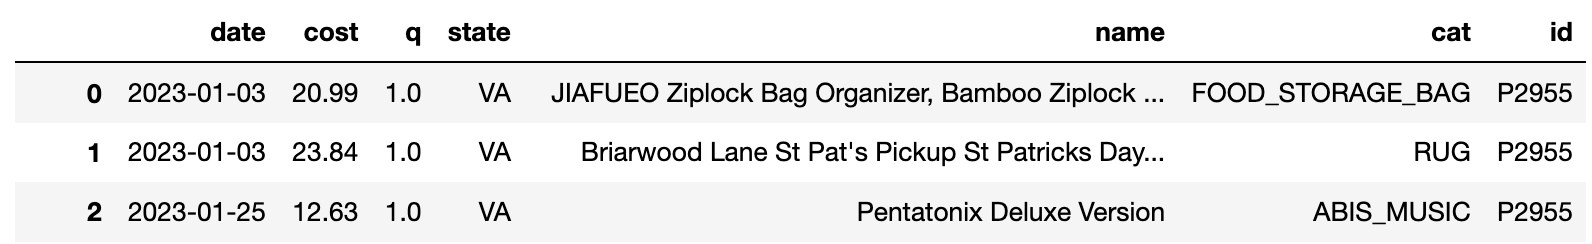
\includegraphics[width=1\textwidth]{final-images/df.png}

\end{center}

\vspace{.1in}

\noindent The columns in \texttt{skin} are as follows:

\begin{itemize}

\item{\texttt{"Type" (str)}: The type of product. There are six different possible types, three of which are shown above.}
\item{\texttt{"Brand" (str)}: The brand of the product. As shown above, brands can have multiple products.}
\item{\texttt{"Name" (str)}: The name of product. Assume that product names are unique.}
\item{\texttt{"Price" (int)}: The price of the product, in a whole number of dollars.}
\item{\texttt{"Rating" (float)}: The rating of the product on \texttt{sephora.com}; ranges from \texttt{0.0} to \texttt{5.0}.}
\item{\texttt{"Num Ingredients" (int)}: The number of ingredients in the product.}
\item{\texttt{"Sensitive" (int)}: \texttt{1} if the product is made for individuals with sensitive skin, and \texttt{0} otherwise.}

\end{itemize}


\noindent \textbf{Throughout the exam}, assume we have already run all necessary import statements.

\newpage

\noindent \textbf{Make sure you have read the Data Overview \textit{and} read all of the questions on the exam before you start writing!}

\begin{probset}

\begin{prob}[(8 pts) \small{\boxed{\text{Counts towards midterm redemption}}}]

\vspace{0.1in}

An expensive product is one that costs \textbf{at least \$100}.

%TOVERSION: Expensive threshold, maybe change to cheap.

\begin{subprobset}

\begin{subprob}(3 pts) Fill in the blank below with an expression that evaluates to the \textbf{proportion} of products in \texttt{skin} that are expensive.

\biginlineresponsebox[6in]{}

\end{subprob}

\vspace{0.2in}

\begin{subprob}(5 pts) Fill in the blanks so that the expression below evaluates to the number of brands that sell \textbf{fewer than 5} expensive products.

\begin{verbatim}

skin.groupby(__(i)__).__(ii)__(__(iii)__)["Brand"].nunique()

\end{verbatim}

\texttt{(i)}: 

\bubble{\texttt{"Brand"}} 
\bubble{\texttt{"Name"}} 
\bubble{\texttt{"Price"}} 
\bubble{\texttt{["Brand", "Price"]}}

\texttt{(ii)}: 

\bubble{\texttt{agg}}

\bubble{\texttt{count}}

\bubble{\texttt{filter}}

\bubble{\texttt{value\_counts}}

\texttt{(iii)}: \biginlineresponsebox[6in]{}

\end{subprob}

% \vspace{0.2in}

% \begin{subprob}(4 pts) Fill in the blanks so that the expression below \textit{also} evaluates to the number of brands that sell at least 5 expensive products.

% \begin{verbatim}

% (skin.loc[__(i)__].__(ii)__() >= 5).sum()

% \end{verbatim}

% \texttt{(i)}: \hspace{0.02in} \biginlineresponsebox[6in]{}

% \vspace{0.1in}

% \texttt{(ii)}: \bubble{\texttt{agg}} \bubble{\texttt{count}} \bubble{\texttt{filter}} \bubble{\texttt{value\_counts}}

% \end{subprob}

\end{subprobset}
    
\end{prob}

\vspace{1in}

\begin{prob}[(2 pts) \small{\boxed{\text{Counts towards midterm redemption}}}]

Fill in each blank with \textbf{one word} to complete the sentence below.

The SQL keyword for filtering after grouping is \_\_(i)\_\_, and the SQL keyword for querying is \_\_(ii)\_\_.

(i): \inlineresponsebox[3in]{} (ii): \inlineresponsebox[3in]{}

\end{prob}

\newpage

\begin{prob}[(9 pts) \small{\boxed{\text{Counts towards midterm redemption}}}]

Consider the Series \texttt{small\_prices} and \texttt{vc}, both of which are defined below.

\begin{verbatim}

small_prices = pd.Series([
    36, 36, 18, 100, 18, 36, 1, 1, 1, 36]
])

vc = small_prices.value_counts().sort_values(ascending=False)

\end{verbatim}

% Consider the Series \texttt{vc}, defined below. 

% \begin{verbatim}
% vc = 
% \end{verbatim}

In each of the parts below, select the value that the provided expression evaluates to. If the expression errors, select ``Error".

\begin{subprobset}

\begin{subprob}(1.5 pts) \texttt{vc.iloc[0]}?

\begin{tabular}{lllll}

\bubble{\texttt{0}} & 

\bubble{\texttt{1}} & 

\bubble{\texttt{2}} & 

\bubble{\texttt{3}} & 

\bubble{\texttt{4}} \\ 

\bubble{\texttt{18}} & 

\bubble{\texttt{36}} & 

\bubble{\texttt{100}} &

\bubble{Error} & 

\bubble{None of these}
\end{tabular}

\end{subprob}

\vspace{0.1in}

\begin{subprob}(1.5 pts) \texttt{vc.loc[0]}

\begin{tabular}{lllll}

\bubble{\texttt{0}} & 

\bubble{\texttt{1}} & 

\bubble{\texttt{2}} & 

\bubble{\texttt{3}} & 

\bubble{\texttt{4}} \\ 

\bubble{\texttt{18}} & 

\bubble{\texttt{36}} & 

\bubble{\texttt{100}} &

\bubble{Error} & 

\bubble{None of these}
\end{tabular}

\end{subprob}

\vspace{0.1in}

\begin{subprob}(1.5 pts) \texttt{vc.index[0]}

\begin{tabular}{lllll}

\bubble{\texttt{0}} & 

\bubble{\texttt{1}} & 

\bubble{\texttt{2}} & 

\bubble{\texttt{3}} & 

\bubble{\texttt{4}} \\ 

\bubble{\texttt{18}} & 

\bubble{\texttt{36}} & 

\bubble{\texttt{100}} &

\bubble{Error} & 

\bubble{None of these}
\end{tabular}

\end{subprob}

\vspace{0.1in}

\begin{subprob}(1.5 pts) \texttt{vc.iloc[1]}

\begin{tabular}{lllll}

\bubble{\texttt{0}} & 

\bubble{\texttt{1}} & 

\bubble{\texttt{2}} & 

\bubble{\texttt{3}} & 

\bubble{\texttt{4}} \\ 

\bubble{\texttt{18}} & 

\bubble{\texttt{36}} & 

\bubble{\texttt{100}} &

\bubble{Error} & 

\bubble{None of these}
\end{tabular}

\end{subprob}

\vspace{0.1in}

\begin{subprob}(1.5 pts) \texttt{vc.loc[1]}

\begin{tabular}{lllll}

\bubble{\texttt{0}} & 

\bubble{\texttt{1}} & 

\bubble{\texttt{2}} & 

\bubble{\texttt{3}} & 

\bubble{\texttt{4}} \\ 

\bubble{\texttt{18}} & 

\bubble{\texttt{36}} & 

\bubble{\texttt{100}} &

\bubble{Error} & 

\bubble{None of these}
\end{tabular}

\end{subprob}

\vspace{0.1in}

\begin{subprob}(1.5 pts) \texttt{vc.index[1]}

\begin{tabular}{lllll}

\bubble{\texttt{0}} & 

\bubble{\texttt{1}} & 

\bubble{\texttt{2}} & 

\bubble{\texttt{3}} & 

\bubble{\texttt{4}} \\ 

\bubble{\texttt{18}} & 

\bubble{\texttt{36}} & 

\bubble{\texttt{100}} &

\bubble{Error} & 

\bubble{None of these}
\end{tabular}

\end{subprob}

\end{subprobset}

\end{prob}

\newpage

\begin{prob}[(6 pts) \small{\boxed{\text{Counts towards midterm redemption}}}]

Consider the DataFrames \texttt{type\_pivot}, \texttt{clinique}, \texttt{fresh}, and \texttt{boscia}, defined below.

\begin{verbatim}

type_pivot = skin.pivot_table(index="Type",
                              columns="Brand", 
                              values="Sensitive",
                              aggfunc=lambda s: s.shape[0] + 1)
                               
clinique = skin[skin["Brand"] == "CLINIQUE"]
fresh = skin[skin["Brand"] == "FRESH"]
boscia = skin[skin["Brand"] == "BOSCIA"]

\end{verbatim}

Three columns of \texttt{type\_pivot} are shown below \textbf{in their entirety}.

\vspace{-0.05in}

\begin{center}

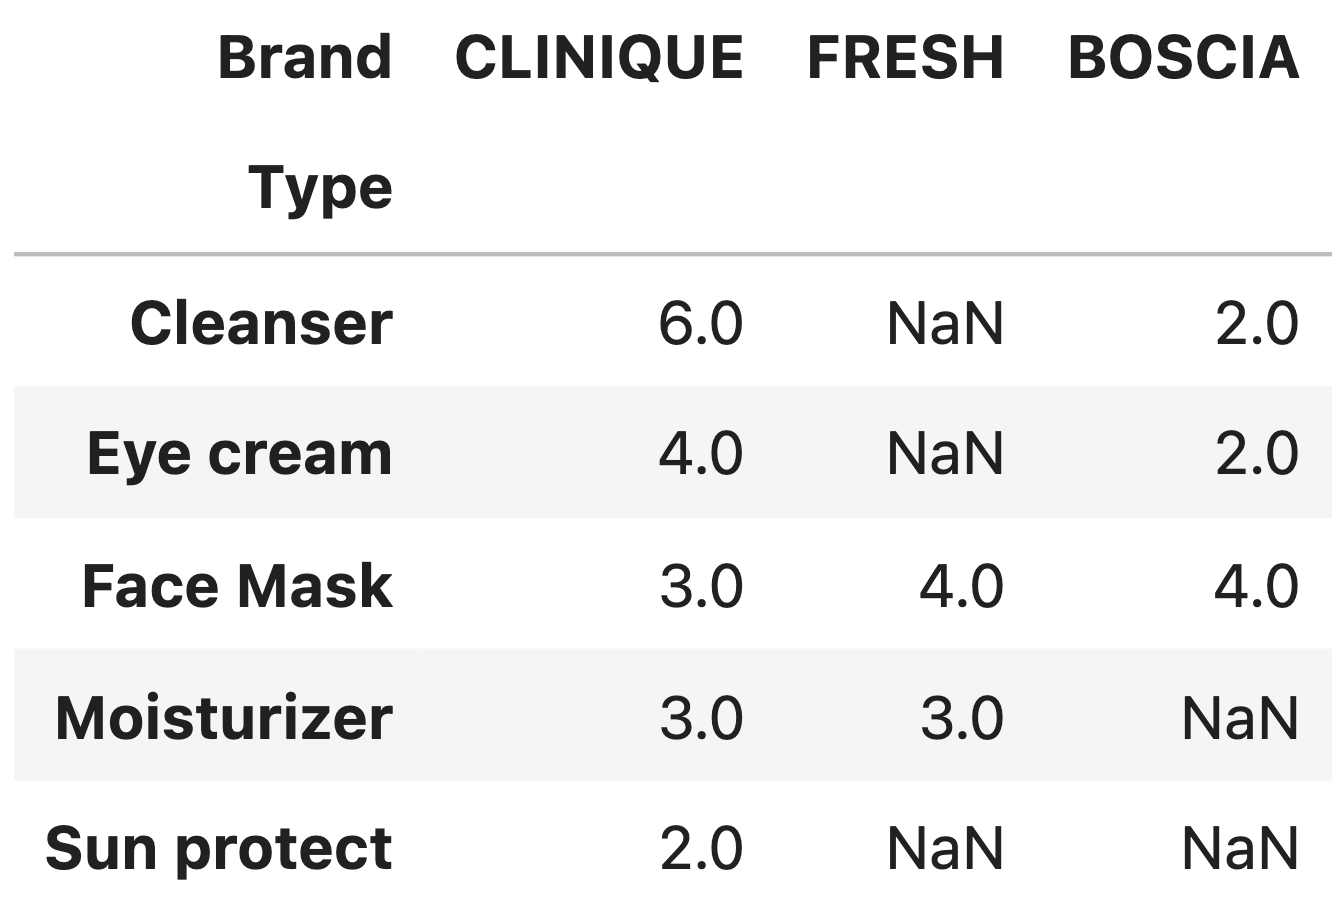
\includegraphics[width=0.5\textwidth]{final-images/type-pivot.png}

\end{center}

In each of the parts below, give your answer as an \textbf{integer}.

\begin{subprobset}

\begin{subprob}(3 pts) How many rows are in the following DataFrame?

\begin{verbatim}
clinique.merge(fresh, on="Type", how="inner")
\end{verbatim}

\inlineresponsebox[1.25in]{}

% \bubble{9} \bubble{10} \bubble{11} \bubble{12} \bubble{13} \bubble{18} \bubble{21}

\end{subprob}

% \begin{subprob}

% How many rows are in the following DataFrame?

% \begin{verbatim}
% fresh.merge(boscia, on="Type", how="right")
% \end{verbatim}

% \bubble{9} \bubble{10} \bubble{11} \bubble{12} \bubble{13} \bubble{18} \bubble{21}


% \end{subprob}

\begin{subprob}(3 pts) How many rows are in the following DataFrame?

\begin{verbatim}
(clinique.merge(fresh, on="Type", how="outer")
         .merge(boscia, on="Type", how="outer"))
\end{verbatim}

\inlineresponsebox[1.25in]{}

% \bubble{12} \bubble{13} \bubble{18} \bubble{21} \bubble{29} \bubble{32} \bubble{34}

\end{subprob}

\end{subprobset}

\end{prob}

\newpage

\begin{prob}[(5 pts) \small{\boxed{\text{Counts towards midterm redemption}}}]

Consider a sample of 60 skincare products. The name of one product from the sample is given below:

\begin{center}
``our \textbf{drops} cream is the best \textbf{drops} \textbf{drops} for eye \textbf{drops} \textbf{drops} proven formula..."
\end{center}

The total number of terms in the product name above is unknown, but we know that the term \textbf{drops} only appears in the name 5 times.

\vspace{0.1in}

Suppose the TF-IDF of \texttt{drops} in the product name above is $\frac{2}{3}$. Which of the following statements are \textbf{NOT possible}, assuming we use a base-2 logarithm? Select all that apply.

\vspace{0.1in}

\squarebubble{\textbf{All} 60 product names contain the term \texttt{drops}, \textbf{including} the one above.}

\squarebubble{14 \textbf{other} product names contain the term \texttt{drops}, in addition to the one above.}

\squarebubble{None of the 59 \textbf{other} product names contain the term \texttt{drops}.}

\squarebubble{There are 15 terms in the product name above \textbf{in total}.}

\correctsquarebubble{There are 25 terms in the product name above \textbf{in total}.}

\end{prob}

\vspace{0.2in}

\newpage

\begin{prob}[(3 pts) \small{\boxed{\text{Counts towards midterm redemption}}}]

Suppose \texttt{soup} is a BeautifulSoup object representing the homepage of \texttt{wolfskin.com}, a Sephora competitor.

Furthermore, suppose \texttt{prods}, defined below, is a list of strings containing the name of every product on the site.

\begin{verbatim}
prods = [row.get("prod") for row in soup.find_all("row", class_="thing")]
\end{verbatim}

Given that \texttt{prods[1]} evaluates to \texttt{"Cleansifier"}, which of the following options describes the source code of \texttt{wolfskin.com}?

\vspace{0.3in}

\begin{itemize}

\item Option 1:

\begin{verbatim}
<row class="thing">prod: Facial Treatment Essence</row>
<row class="thing">prod: Cleansifier</row>
<row class="thing">prod: Self Tan Dry Oil SPF 50</row>
...
\end{verbatim}

\vspace{0.1in}

\item Option 2:

\begin{verbatim}
<row class="thing" prod="Facial Treatment Essence"></row>
<row class="thing" prod="Cleansifier"></row>
<row class="thing" prod="Self Tan Dry Oil SPF 50"></row>
...
\end{verbatim}

\vspace{0.1in}

\item Option 3:

\begin{verbatim}
<row prod="thing" class="Facial Treatment Essence"></row>
<row prod="thing" class="Cleansifier"></row>
<row prod="thing" class="Self Tan Dry Oil SPF 50"></row>
...
\end{verbatim}

\vspace{0.1in}

\item Option 4:

\begin{verbatim}
<row class="thing">prod="Facial Treatment Essence"</row>
<row class="thing">prod="Cleansifier"</row>
<row class="thing">prod="Self Tan Dry Oil SPF 50"</row>
...
\end{verbatim}

\vspace{0.1in}

\end{itemize}

\bubble{Option 1} 

\bubble{Option 2} 

\bubble{Option 3} 

\bubble{Option 4}

\end{prob}

\newpage

\begin{prob}[(13 pts)]

Consider a dataset of $n$ values, $y_1, y_2, ..., y_n$, all of which are \textbf{positive}. We want to fit a constant model, $H(x) = h$, to the data.

Let $h_p^*$ be the optimal constant prediction that minimizes average degree-$p$ loss, $R_p(h)$, defined below.

$$R_p(h) = \frac{1}{n} \sum_{i = 1}^n | y_i - h |^p$$

\vspace{-0.2in}

For example, $h_2^*$ is the optimal constant prediction that minimizes $\displaystyle R_2(h) = \frac{1}{n} \sum_{i = 1}^n |y_i - h|^2$.

In each of the parts below, determine the value of the quantity provided. By ``the data", we are referring to $y_1, y_2, ..., y_n$.

\begin{subprobset}

\begin{subprob}(1.5 pts) $h_0^*$

\begin{tabular}{ll}

\bubble{The standard deviation of the data} 

\bubble{The variance of the data}
\\ 
\bubble{The mean of the data} 

\bubble{The median of the data} \\

\bubble{The midrange of the data, $\frac{y_\text{min} + y_\text{max}}{2}$} 

\bubble{The mode of the data} \\

\bubble{None of the above}

\end{tabular}

\end{subprob}

\begin{subprob}(1.5 pts) $h_1^*$

\begin{tabular}{ll}

    \bubble{The standard deviation of the data} 

    \bubble{The variance of the data}
    \\ 
    \bubble{The mean of the data} 
    
    \bubble{The median of the data} \\
    
    \bubble{The midrange of the data, $\frac{y_\text{min} + y_\text{max}}{2}$} 
    
    \bubble{The mode of the data} \\
    
    \bubble{None of the above}

\end{tabular}

\end{subprob}

\begin{subprob}(1.5 pts) $R_1(h_1^*)$

\begin{tabular}{ll}

    \bubble{The standard deviation of the data} 

    \bubble{The variance of the data}
    \\ 
    \bubble{The mean of the data} 
    
    \bubble{The median of the data} \\
    
    \bubble{The midrange of the data, $\frac{y_\text{min} + y_\text{max}}{2}$} 
    
    \bubble{The mode of the data} \\
    
    \bubble{None of the above}

\end{tabular}

\end{subprob}

\begin{subprob}(1.5 pts) $h_2^*$

\begin{tabular}{ll}

    \bubble{The standard deviation of the data} 

    \bubble{The variance of the data}
    \\ 
    \bubble{The mean of the data} 
    
    \bubble{The median of the data} \\
    
    \bubble{The midrange of the data, $\frac{y_\text{min} + y_\text{max}}{2}$} 
    
    \bubble{The mode of the data} \\
    
    \bubble{None of the above}

\end{tabular}

\end{subprob}

\begin{subprob}(1.5 pts) $R_2(h_2^*)$

\begin{tabular}{ll}

    \bubble{The standard deviation of the data} 

    \bubble{The variance of the data}
    \\ 
    \bubble{The mean of the data} 
    
    \bubble{The median of the data} \\
    
    \bubble{The midrange of the data, $\frac{y_\text{min} + y_\text{max}}{2}$} 
    
    \bubble{The mode of the data} \\
    
    \bubble{None of the above}

\end{tabular}

\end{subprob}

\end{subprobset}

\newpage

Now, suppose we want to find the optimal constant prediction, $h_\text{U}^*$, using the ``Ulta" loss function, defined below.

\vspace{-0.1in}

$$L_U(y_i, h) = y_i (y_i - h)^2$$

\begin{subprobset}

\begin{subprob}(1.5 pts) To find $h_\text{U}^*$, suppose we minimize average Ulta loss (with no regularization). How does $h_\text{U}^*$ compare to the mean of the data, $M$?

\bubble{$h_\text{U}^* > M$} 

\bubble{$h_\text{U}^* \geq M$} 

\bubble{$h_\text{U}^* = M$} 

\bubble{$h_\text{U}^* \leq M$} 

\bubble{$h_\text{U}^* < M$}

\end{subprob}

\end{subprobset}

Now, to find the optimal constant prediction, we will instead minimize \textbf{regularized} average Ulta loss, $R_\lambda(h)$, where $\lambda$ is a non-negative regularization hyperparameter:

$$R_\lambda(h) = \left( \frac{1}{n} \sum_{i = 1}^n y_i (y_i - h)^2 \right) + \lambda h^2$$

It can be shown that $\displaystyle \frac{\partial R_\lambda(h)}{\partial h}$, the derivative of $R_\lambda(h)$ with respect to $h$, is:

$$\frac{\partial R_\lambda(h)}{\partial h} = -2 \left( \frac{1}{n} \sum_{i = 1}^n y_i (y_i - h) - \lambda h \right)$$

\begin{subprobset}

\begin{subprob}(4 pts) Find $h^*$, the constant prediction that minimizes $R_\lambda(h)$. Show your work, and put a \boxed{\text{box}} around your final answer, which should be an \textbf{expression in terms of $y_i$, $n$, and/or $\lambda$}.

\begin{responsebox}{3.8in}
    
\end{responsebox}

\end{subprob}

\end{subprobset}

\end{prob}

\newpage

\begin{prob}[(8 pts)]

Suppose we want to fit a simple linear regression model (using squared loss) that predicts the number of ingredients in a product given its price. We're given that:

\begin{itemize}
    \item The average cost of a product in our dataset is \$40, i.e. $\bar x = 40$.
    \item The average number of ingredients in a product in our dataset is 15, i.e. $\bar y = 15$.
\end{itemize}

The intercept and slope of the regression line are $w_0^* = 11$ and $w_1^* = \frac{1}{10}$, respectively.

\begin{subprobset}

\begin{subprob}(3 pts) Suppose Victors' Veil (a skincare product) costs \$40 and has 11 ingredients. What is the squared loss of our model's predicted number of ingredients for Victors' Veil? Give your answer as a \textbf{number}.

\inlineresponsebox[1.5in]{}

\end{subprob}

\vspace{0.25in}

\begin{subprob}(2 pts) Is it possible to answer part (a) above \textbf{just} by knowing $\bar x$ and $\bar y$, i.e. \textbf{without} knowing the values of $w_0^*$ and $w_1^*$?

\bubble{Yes; the values of $w_0^*$ and $w_1^*$ don't impact the answer to part (a).}

\bubble{No; the values of $w_0^*$ and $w_1^*$ are necessary to answer part (a).}

\end{subprob}

\vspace{0.25in}

\begin{subprob}(3 pts) Suppose $x_i$ represents the price of product $i$, and suppose $u_i$ represents the \textbf{negative price} of product $i$. In other words, for $i = 1, 2, ..., n$, where $n$ is the number of points in our dataset:

$$u_i = - x_i$$

% Let $\beta_0^*$ and $\beta_1^*$ be the intercept and slope, respectively, of the regression line that predicts $y$ given $u$. Give both answers below as \textbf{numbers} (with no variables).

% \begin{enumerate}[label=(\roman*)]

% \item What is the value of $\beta_0^*$, the \textbf{intercept} of the new regression line?

% \biginlineresponsebox[1.5in]{}

% \item What is the value of $\beta_1^*$, the \textbf{slope} of the new regression line?

% \biginlineresponsebox[1.5in]{}

% \end{enumerate}

% \end{subprob}

% \newpage

% \begin{subprob}(2 pts) 

Suppose $U$ is the design matrix for the simple linear regression model that uses \textbf{negative} price to predict number of ingredients. Which of the following matrices could be $U^TU$?

\vspace{0.1in}

\begin{tabular}{ll}

\bubble{\begin{bmatrix} -15 & 600 \\ 600 & -30000 \end{bmatrix}}

\bubble{\begin{bmatrix} 15 & -600 \\ -600 & 30000 \end{bmatrix}}

\bubble{\begin{bmatrix} -15 & 450 \\ 450 & -30000 \end{bmatrix}}

\bubble{\begin{bmatrix} 15 & -450 \\ -450 & 30000 \end{bmatrix}}

\end{tabular}

\end{subprob}

\end{subprobset}
    
\end{prob}

\newpage

\begin{prob}[(8 pts)]

Suppose we want to fit a multiple linear regression model (using squared loss) that predicts the number of ingredients in a product given its price and various other information.

From the Data Overview page, we know that there are \textbf{6} different \textbf{types} of products. Assume in this question that there are \textbf{20} different product \textbf{brands}. Consider the models defined in the table below.

\begin{table}[h!]
\centering
\renewcommand{\arraystretch}{1}
\setlength{\tabcolsep}{8pt}
\begin{tabular}{|c|c|c|c|c|}
\hline
\textbf{Model Name} & \textbf{Intercept} & \textbf{Price} & \textbf{Type} & \textbf{Brand} \\ \hline
\textbf{Model A} & Yes & Yes & No & \makecell{One hot encoded \\ \textbf{without} \texttt{drop="first"}} \\ \hline
\textbf{Model B} & Yes & Yes & No & No \\ \hline
\textbf{Model C} & Yes & Yes & \makecell{One hot encoded \\ \textbf{without} \texttt{drop="first"}} & No \\ \hline
\textbf{Model D} & No & Yes & \makecell{One hot encoded \\ \textbf{with} \texttt{drop="first"}} & \makecell{One hot encoded \\ \textbf{with} \texttt{drop="first"}} \\ \hline
\textbf{Model E} & No & Yes & \makecell{One hot encoded \\ \textbf{with} \texttt{drop="first"}} & \makecell{One hot encoded \\ \textbf{without} \texttt{drop="first"}} \\ \hline
\end{tabular}
\end{table}

\vspace{-0.1in}

For instance, Model A above includes an intercept term, price as a feature, one hot encodes brand names, and doesn't use \texttt{drop="first"} as an argument to \texttt{OneHotEncoder} in \texttt{sklearn}.

In parts (a) through (c), you are given a model. For each model provided, state the \textbf{number} of columns and the rank (i.e. number of linearly independent columns) of the design matrix, $X$. Some of part (a) is already done for you as an example.

\begin{subprobset}

\begin{subprob}(1 pt) \textbf{Model A}

Number of columns in $X$: \inlineresponsebox[1in]{22} \hspace{0.3in} Rank of $X$: \boxedinlineresponsebox[1in]{21}

\end{subprob}

\begin{subprob}(2 pts) \textbf{Model B}

Number of columns in $X$: \inlineresponsebox[1in]{2} \hspace{0.3in} Rank of $X$: \inlineresponsebox[1in]{2}

\end{subprob}

\begin{subprob}(2 pts) \textbf{Model C}

Number of columns in $X$: \inlineresponsebox[1in]{8} \hspace{0.3in} Rank of $X$: \inlineresponsebox[1in]{7}

\end{subprob}

% \begin{subprob}(2 pts) \textbf{Model D}

% Number of columns in $X$: \inlineresponsebox[1in]{25} \hspace{0.3in} Rank of $X$: \inlineresponsebox[1in]{25}

% \end{subprob}

% \begin{subprob}(2 pts) \textbf{Model E}

% Number of columns in $X$: \inlineresponsebox[1in]{26} \hspace{0.3in} Rank of $X$: \inlineresponsebox[1in]{26}

% \end{subprob}

% \end{subprobset}

% For your convenience, we repeat the table of models from the previous page below.

% \begin{table}[h!]
% \centering
% \renewcommand{\arraystretch}{1}
% \setlength{\tabcolsep}{8pt}
% \begin{tabular}{|c|c|c|c|c|}
% \hline
% \textbf{Model Name} & \textbf{Intercept} & \textbf{Price} & \textbf{Type} & \textbf{Brand} \\ \hline
% \textbf{Model A} & Yes & Yes & No & \makecell{One hot encoded \\ \textbf{without} \texttt{drop="first"}} \\ \hline
% \textbf{Model B} & Yes & Yes & No & No \\ \hline
% \textbf{Model C} & Yes & Yes & \makecell{One hot encoded \\ \textbf{without} \texttt{drop="first"}} & No \\ \hline
% \textbf{Model D} & No & Yes & \makecell{One hot encoded \\ \textbf{with} \texttt{drop="first"}} & \makecell{One hot encoded \\ \textbf{with} \texttt{drop="first"}} \\ \hline
% \textbf{Model E} & No & Yes & \makecell{One hot encoded \\ \textbf{with} \texttt{drop="first"}} & \makecell{One hot encoded \\ \textbf{without} \texttt{drop="first"}} \\ \hline
% \end{tabular}
% \end{table}

% \begin{subprobset}

\begin{subprob}(3 pts) Which of the following models are \textbf{NOT guaranteed} to have residuals that sum to 0?

\textit{Hint: Remember, the residuals of a fit model are the differences between actual and predicted $y$-values, among the data points in the training set.}

\squarebubble{Model A}

\squarebubble{Model B}

\squarebubble{Model C}

\squarebubble{Model D}

\squarebubble{Model E}

\end{subprob}

\end{subprobset}

\end{prob}

\newpage

\begin{prob}[(5 pts)]

Suppose we want to create polynomial features and use ridge regression (i.e. minimize mean squared error with $L_2$ regularization) to fit a linear model that predicts the number of ingredients in a product given its price.

To choose the polynomial degree and regularization hyperparameter, we use cross-validation through \texttt{GridSearchCV} in \texttt{sklearn} using the code below.

\begin{verbatim}
searcher = GridSearchCV(
    make_pipeline(PolynomialFeatures(include_bias=False), 
                  Ridge()),
    
    param_grid={"polynomialfeatures__degree": np.arange(1, D + 1), 
                "ridge__alpha": 2 ** np.arange(1, L + 1)},

    cv=K # K-fold cross-validation.
) 
searcher.fit(X_train, y_train)
\end{verbatim}

Assume that there are $N$ rows in \texttt{X\_train}, where $N$ is a multiple of $K$ (the number of folds used for cross-validation).

In each of the parts below, give your answer as an \textbf{expression involving $D$, $L$, $K$, and/or $N$}. Part (a) is done for you as an example.

\begin{subprobset}

\begin{subprob}

How many combinations of hyperparameters are being considered?

\fbox{\begin{minipage}[c][0.5in][c]{1.98in}
    \centering
    \( LD \)
\end{minipage}}

\end{subprob}

\begin{subprob}(2.5 pts) \textbf{Each time} a model is trained, how many points are being used to train the model?

\biginlineresponsebox[2in]{}

\end{subprob}

\begin{subprob}(2.5 pts) \textbf{In total}, how many times are \texttt{X\_train.iloc[1]} and \texttt{X\_train.iloc[-1]} \textbf{both} used for training a model \textbf{at the same time}? Assume that these two points are in different folds.

\biginlineresponsebox[2in]{}

\end{subprob}

\end{subprobset}

\end{prob}

% \begin{prob}

% Suppose $X$ is the design matrix and $\lambda$ is a non-negative scalar. Select all true statements below.

% \bubble{$X^TX + n \lambda I$ is only invertible if $X^TX$ is invertible.}

% \bubble{$X^TX$ is only invertible if $X^TX + n \lambda I$ is invertible.}

% \bubble{$X^TX + n \lambda I$ is always invertible, whether or not $X^TX is invertible$.}

% \bubble{$X^TX + n \lambda I$ is always invertible, whether or not $X^TX is invertible$.}

% \end{prob}

\newpage

\begin{prob}[(8 pts)]

Suppose we want to use LASSO (i.e. minimize mean squared error with $L_1$ regularization) to fit a linear model that predicts the number of ingredients in a product given its price and rating.

Let $\lambda$ be a non-negative regularization hyperparameter. Using cross-validation, we determine the average validation mean squared error --- which we'll refer to as AVMSE in this question --- for several different choices of $\lambda$. The results are given below.

\begin{center}

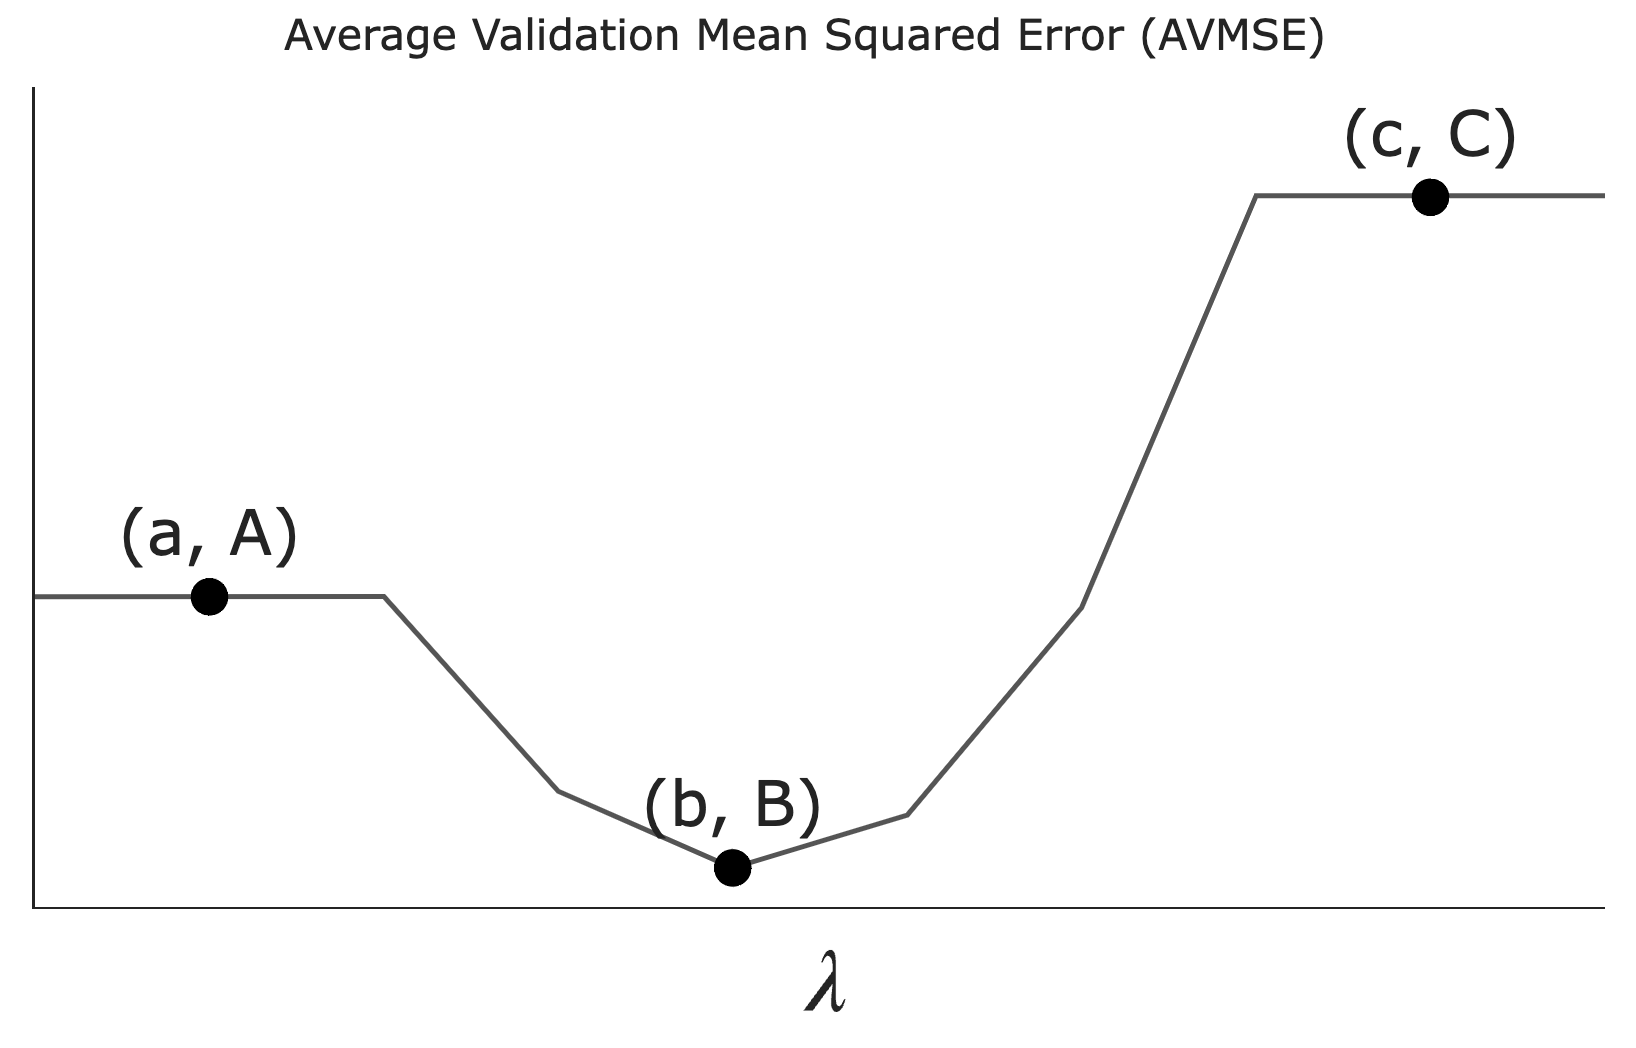
\includegraphics[width=0.7\textwidth]{final-images/avmse.png}

\end{center}

\begin{subprobset}

\begin{subprob}(2 pts) As $\lambda$ increases, what happens to model complexity and model variance?

\bubble{Model complexity and model variance both increase.}

\bubble{Model complexity increases while model variance decreases.}

\bubble{Model complexity decreases while model variance increases.}

\bubble{Model complexity and model variance both decrease.}

\end{subprob}

\begin{subprob}(2 pts) What does the value $A$ on the graph above correspond to?

\bubble{The AVMSE of the $\lambda$ we'd choose to use to train a model.}

\bubble{The AVMSE of an unregularized multiple linear regression model.}

\bubble{The AVMSE of the constant model.}

\end{subprob}

\begin{subprob}(2 pts) What does the value $B$ on the graph above correspond to?

\bubble{The AVMSE of the $\lambda$ we'd choose to use to train a model.}

\bubble{The AVMSE of an unregularized multiple linear regression model.}

\bubble{The AVMSE of the constant model.}

\end{subprob}

\begin{subprob}(2 pts) What does the value $C$ on the graph above correspond to?

\bubble{The AVMSE of the $\lambda$ we'd choose to use to train a model.}

\bubble{The AVMSE of an unregularized multiple linear regression model.}

\bubble{The AVMSE of the constant model.}

\end{subprob}

% \begin{subprob}

% Let $\lambda_\text{cv}$ be the ``best" value of $\lambda$, chosen using cross-validation. Is it guaranteed that $\lambda_\text{cv}$ will lead to the best test set performance?

% \bubble{Yes, no matter what.}

% \bubble{Yes, but only if the test set was produced by calling \texttt{train\_test\_split} on our original dataset.}

% \end{subprob}

\end{subprobset}

\end{prob}

\newpage

% \begin{prob}

% Recall, LASSO regression involves finding the $\vec w^*$ that minimizes mean squared error plus an $L_1$ regularization penalty, while ridge regression involves finding the $\vec w^*$ that minimizes mean squared error plus an $L_2$ regularization.

% Suppose, once again, that we're dealing with a design matrix $X$.

% \begin{subprobset}

% \begin{subprob}

% Feature selection

% \end{subprob}

% \end{subprobset}

% \end{prob}

\newpage

% \begin{subprob}

% Suppose $h^*$ is the constant prediction that minimizes $R_\lambda(h)$, as defined as in the previous part. The residuals of the resulting predictions are:

% $$e_i = y_i - h^*$$

% How can we ensure that the residuals sum to 0, i.e. that $\displaystyle \sum_{i = 1}^n e_i = 0$?

% \bubble{To ensure the residuals sum to 0, set $\lambda = 0$.}

% \bubble{To ensure the residuals sum to 0, set $\lambda$ such that $h^* = \text{Mean}(y_1, y_2, ..., y_n)$.}

% \bubble{To ensure the residuals sum to 0, set $\lambda$ such that $h^* = \text{Variance}(y_1, y_2, ..., y_n)$.}

% \bubble{The residuals always sum to 0, as long as $\lambda \geq 0$.}

% \bubble{For some datasets, no value of $\lambda$ will allow the sum of the residuals to be 0.}
    
% \end{subprob}

% \begin{subprob}

% Now, suppose we have the specific dataset
    
% \end{subprob}

\newpage

\begin{prob}[(6 pts)]

Suppose we fit five different classifiers that predict whether a product is designed for sensitive skin, given its price and number of ingredients. In the five decision boundaries below, the gray-shaded regions represent areas in which the classifier would predict that the product \textbf{is} designed for sensitive skin (i.e. predict class 1). 

\begin{figure}[h!]
    \centering
    % Top row
    \begin{minipage}{0.3\textwidth}
        \centering
        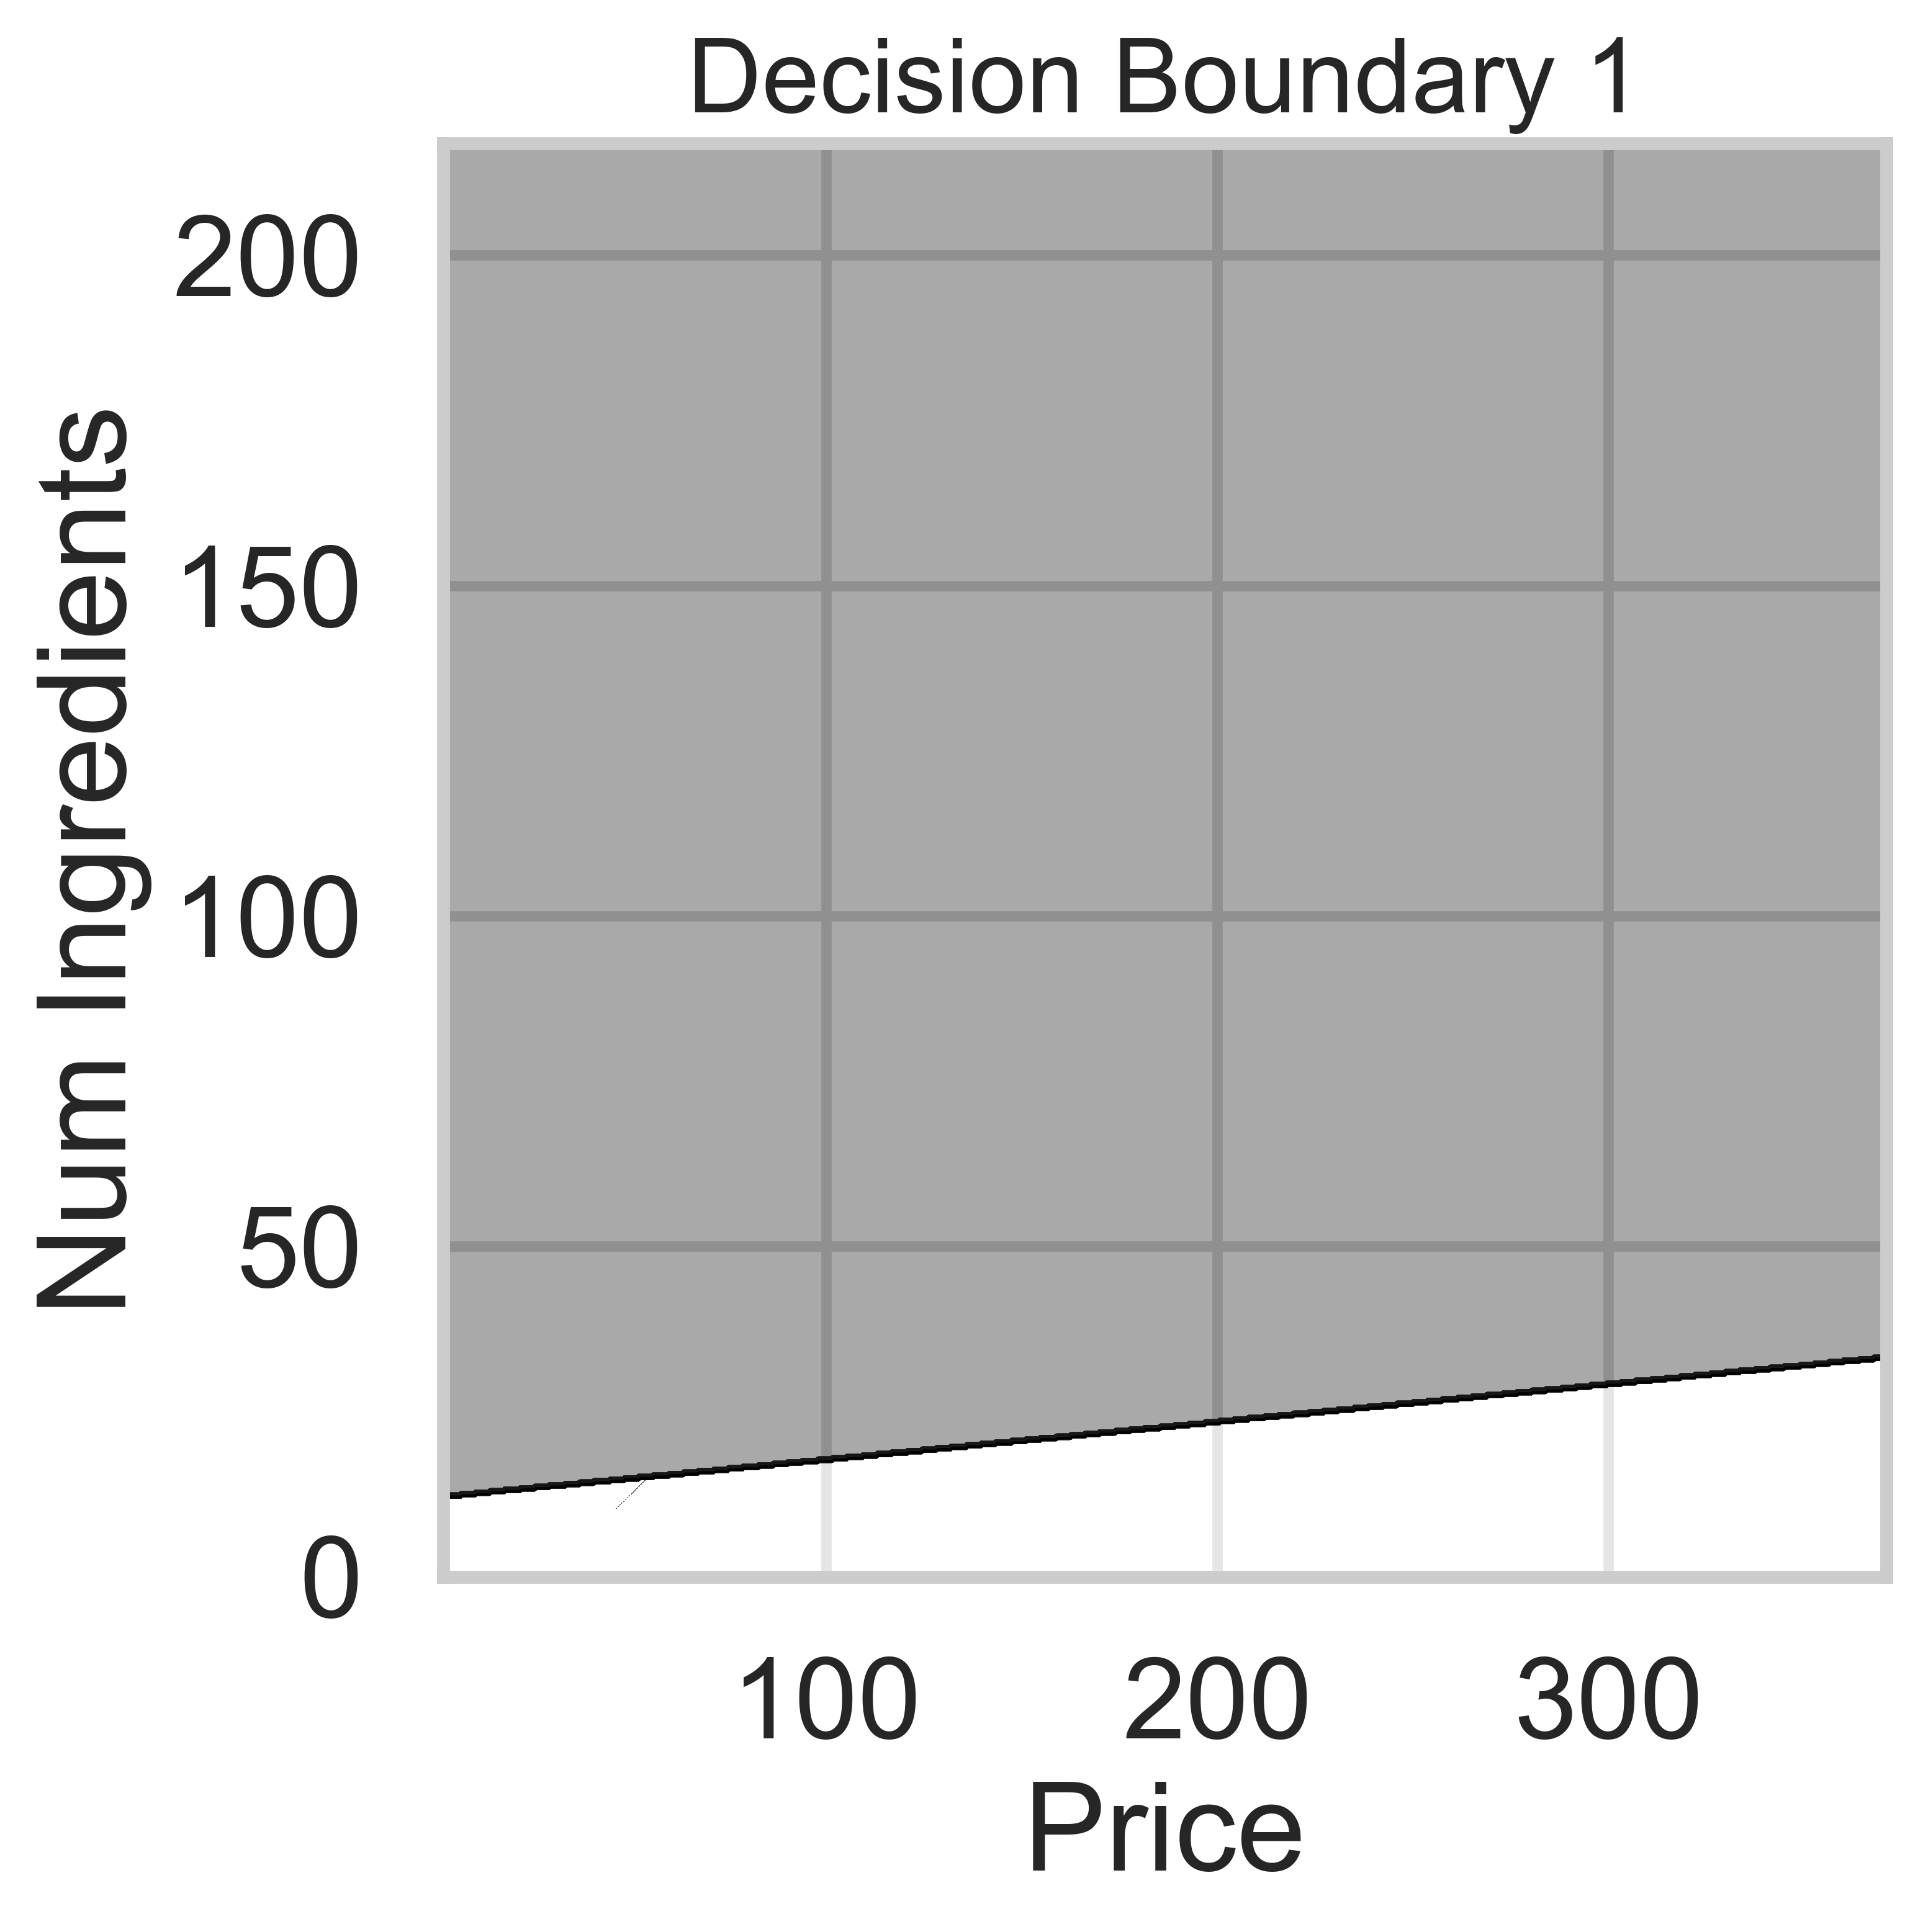
\includegraphics[width=\linewidth]{final-images/db1.png}
    \end{minipage}%
    \hfill
    \begin{minipage}{0.3\textwidth}
        \centering
        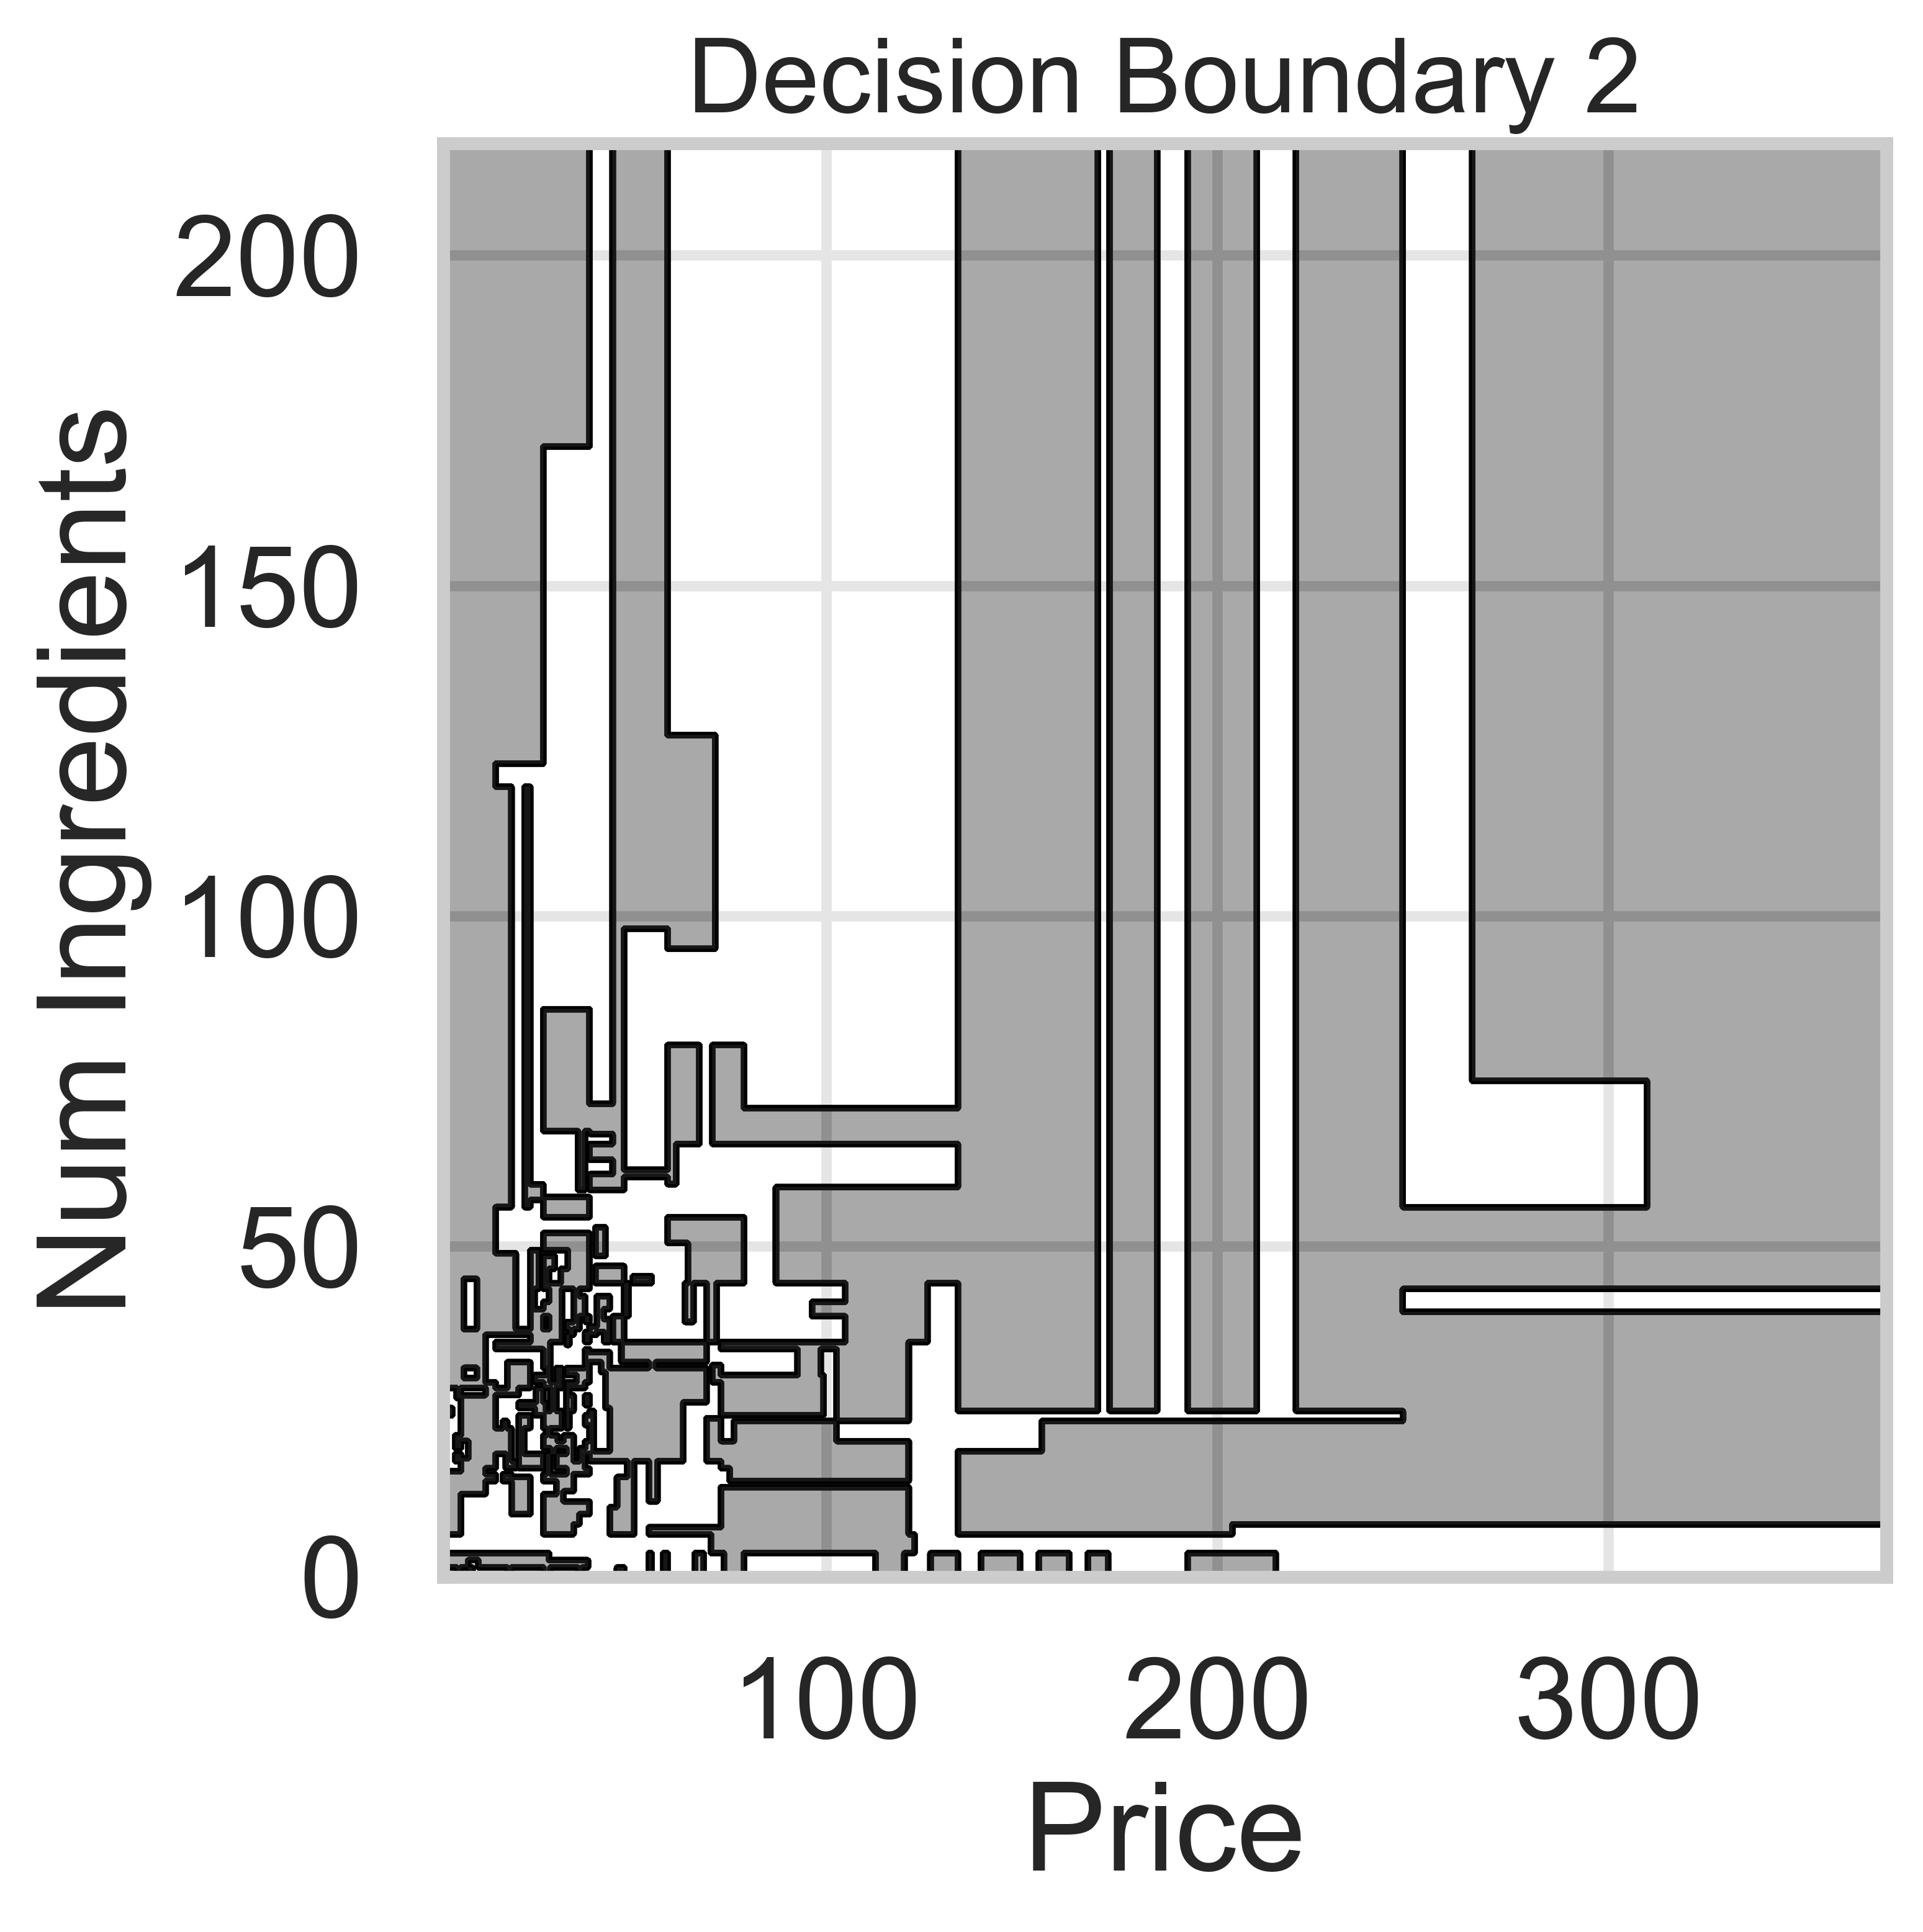
\includegraphics[width=\linewidth]{final-images/db2.png}
    \end{minipage}%
    \hfill
    \begin{minipage}{0.3\textwidth}
        \centering
        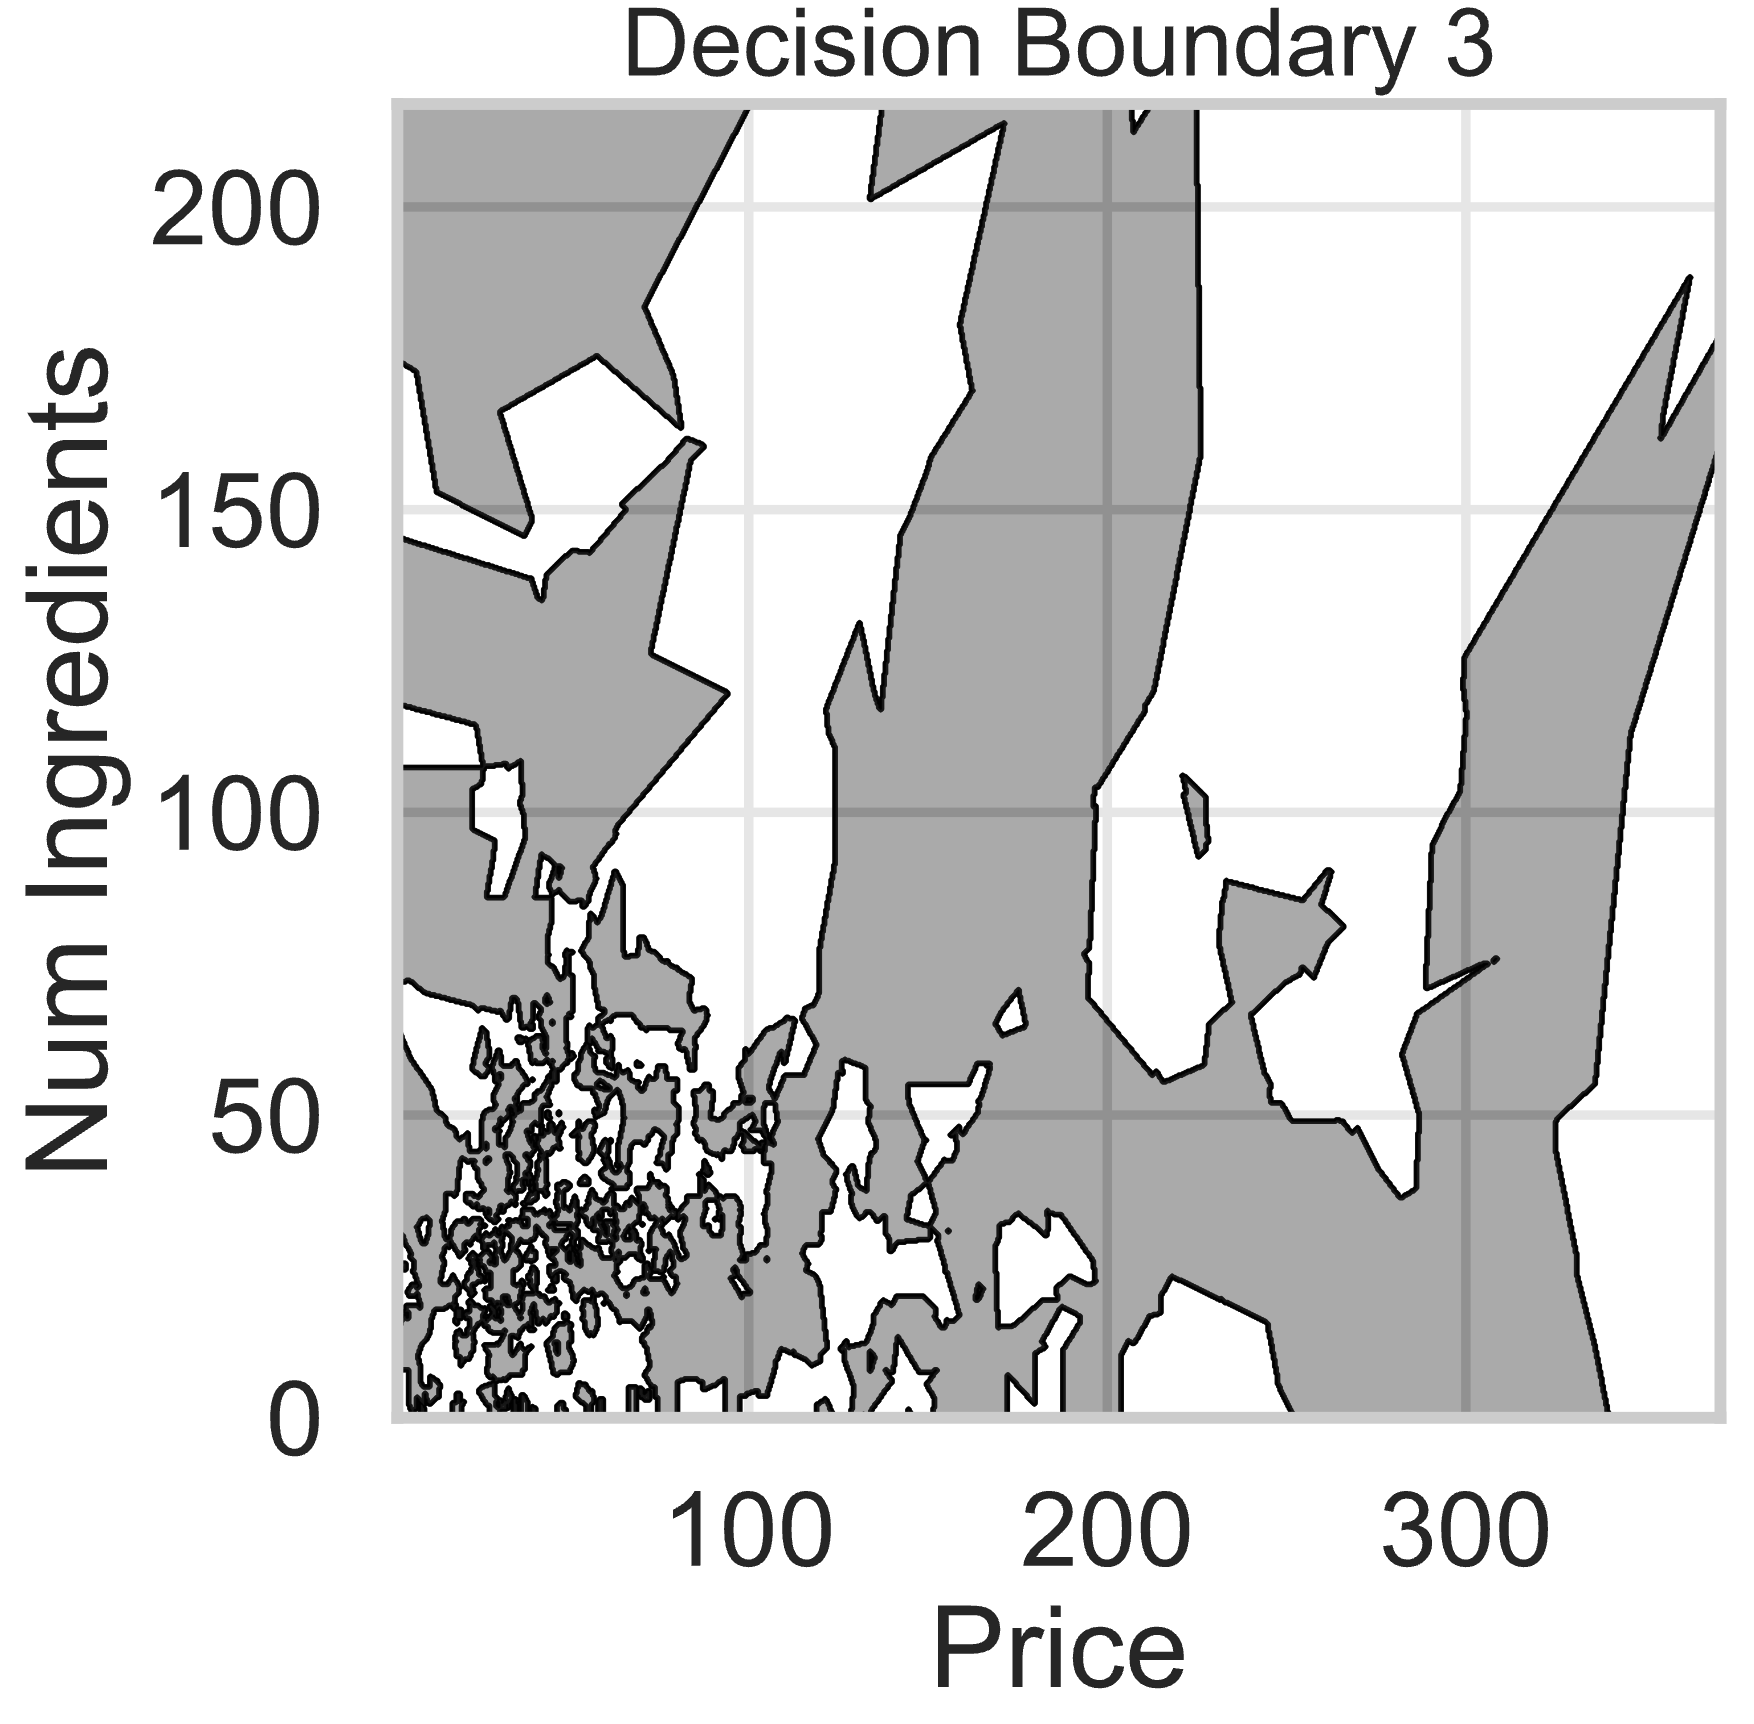
\includegraphics[width=\linewidth]{final-images/db3.png}
    \end{minipage}

    % \vspace{0.3cm} % Add some space between the rows

    % Bottom row
    \begin{minipage}{0.3\textwidth}
        \centering
        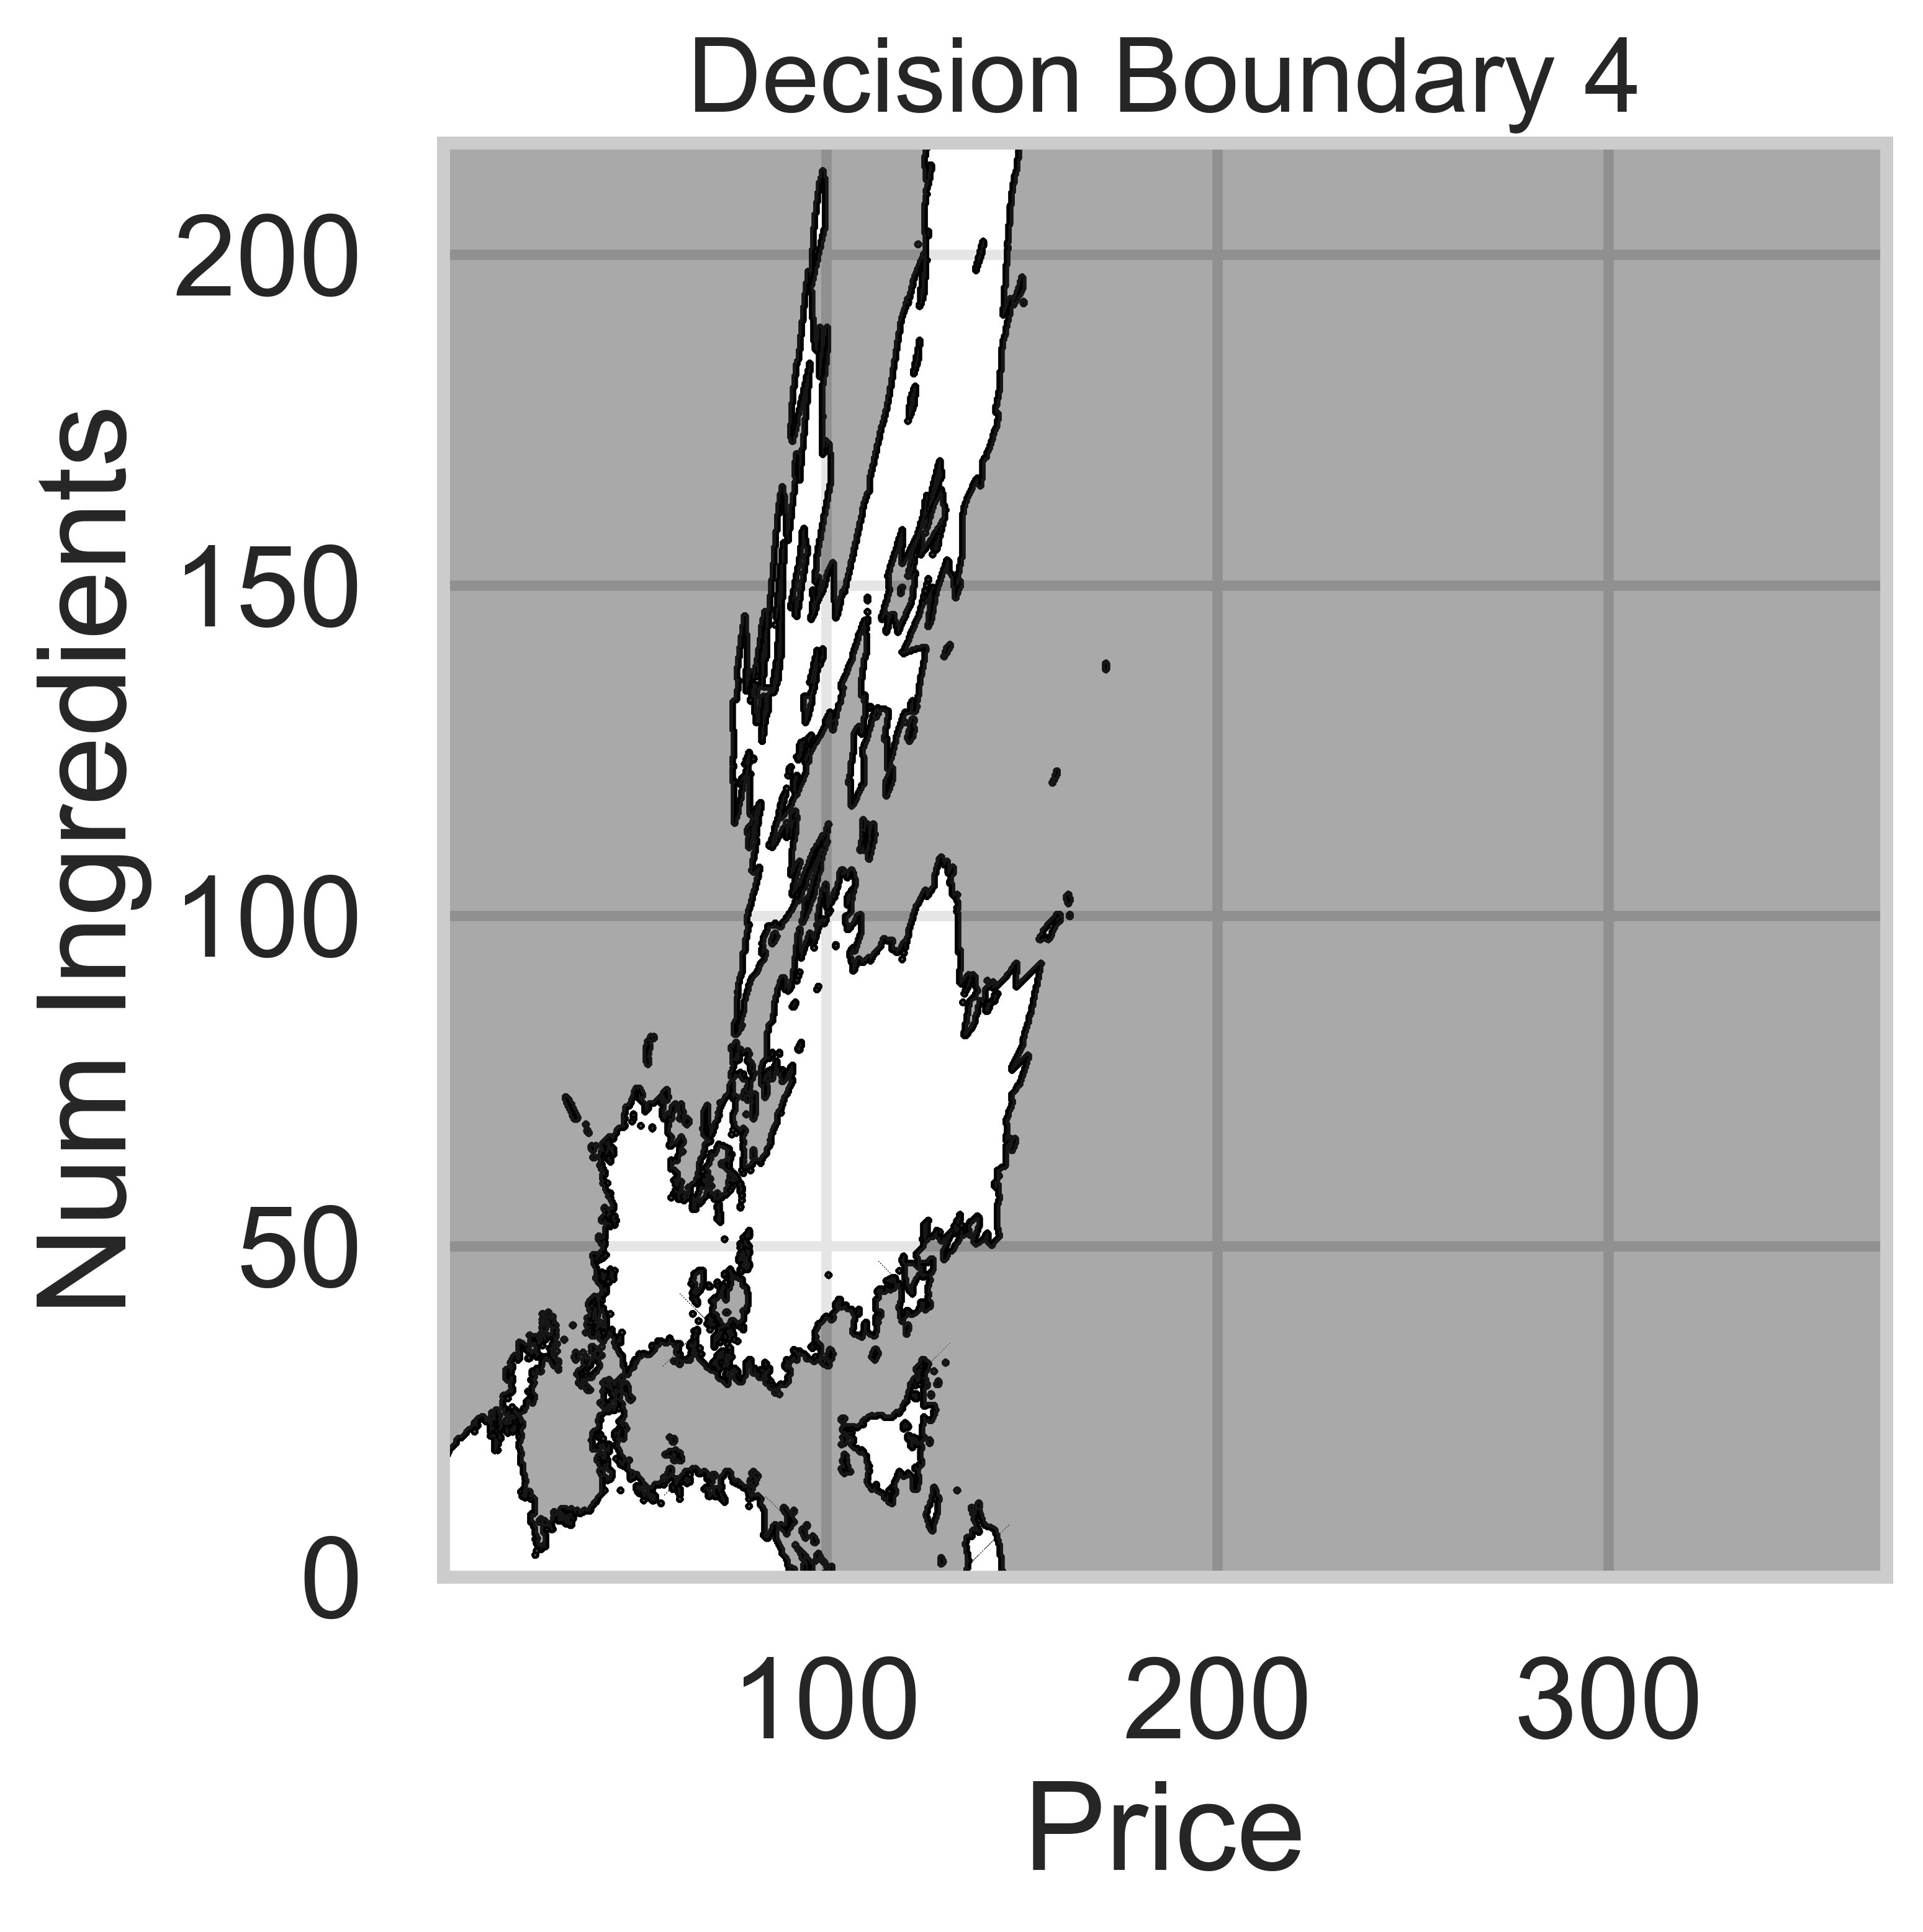
\includegraphics[width=\linewidth]{final-images/db4.png}
    \end{minipage}%
    % \hfill
    \begin{minipage}{0.3\textwidth}
        \centering
        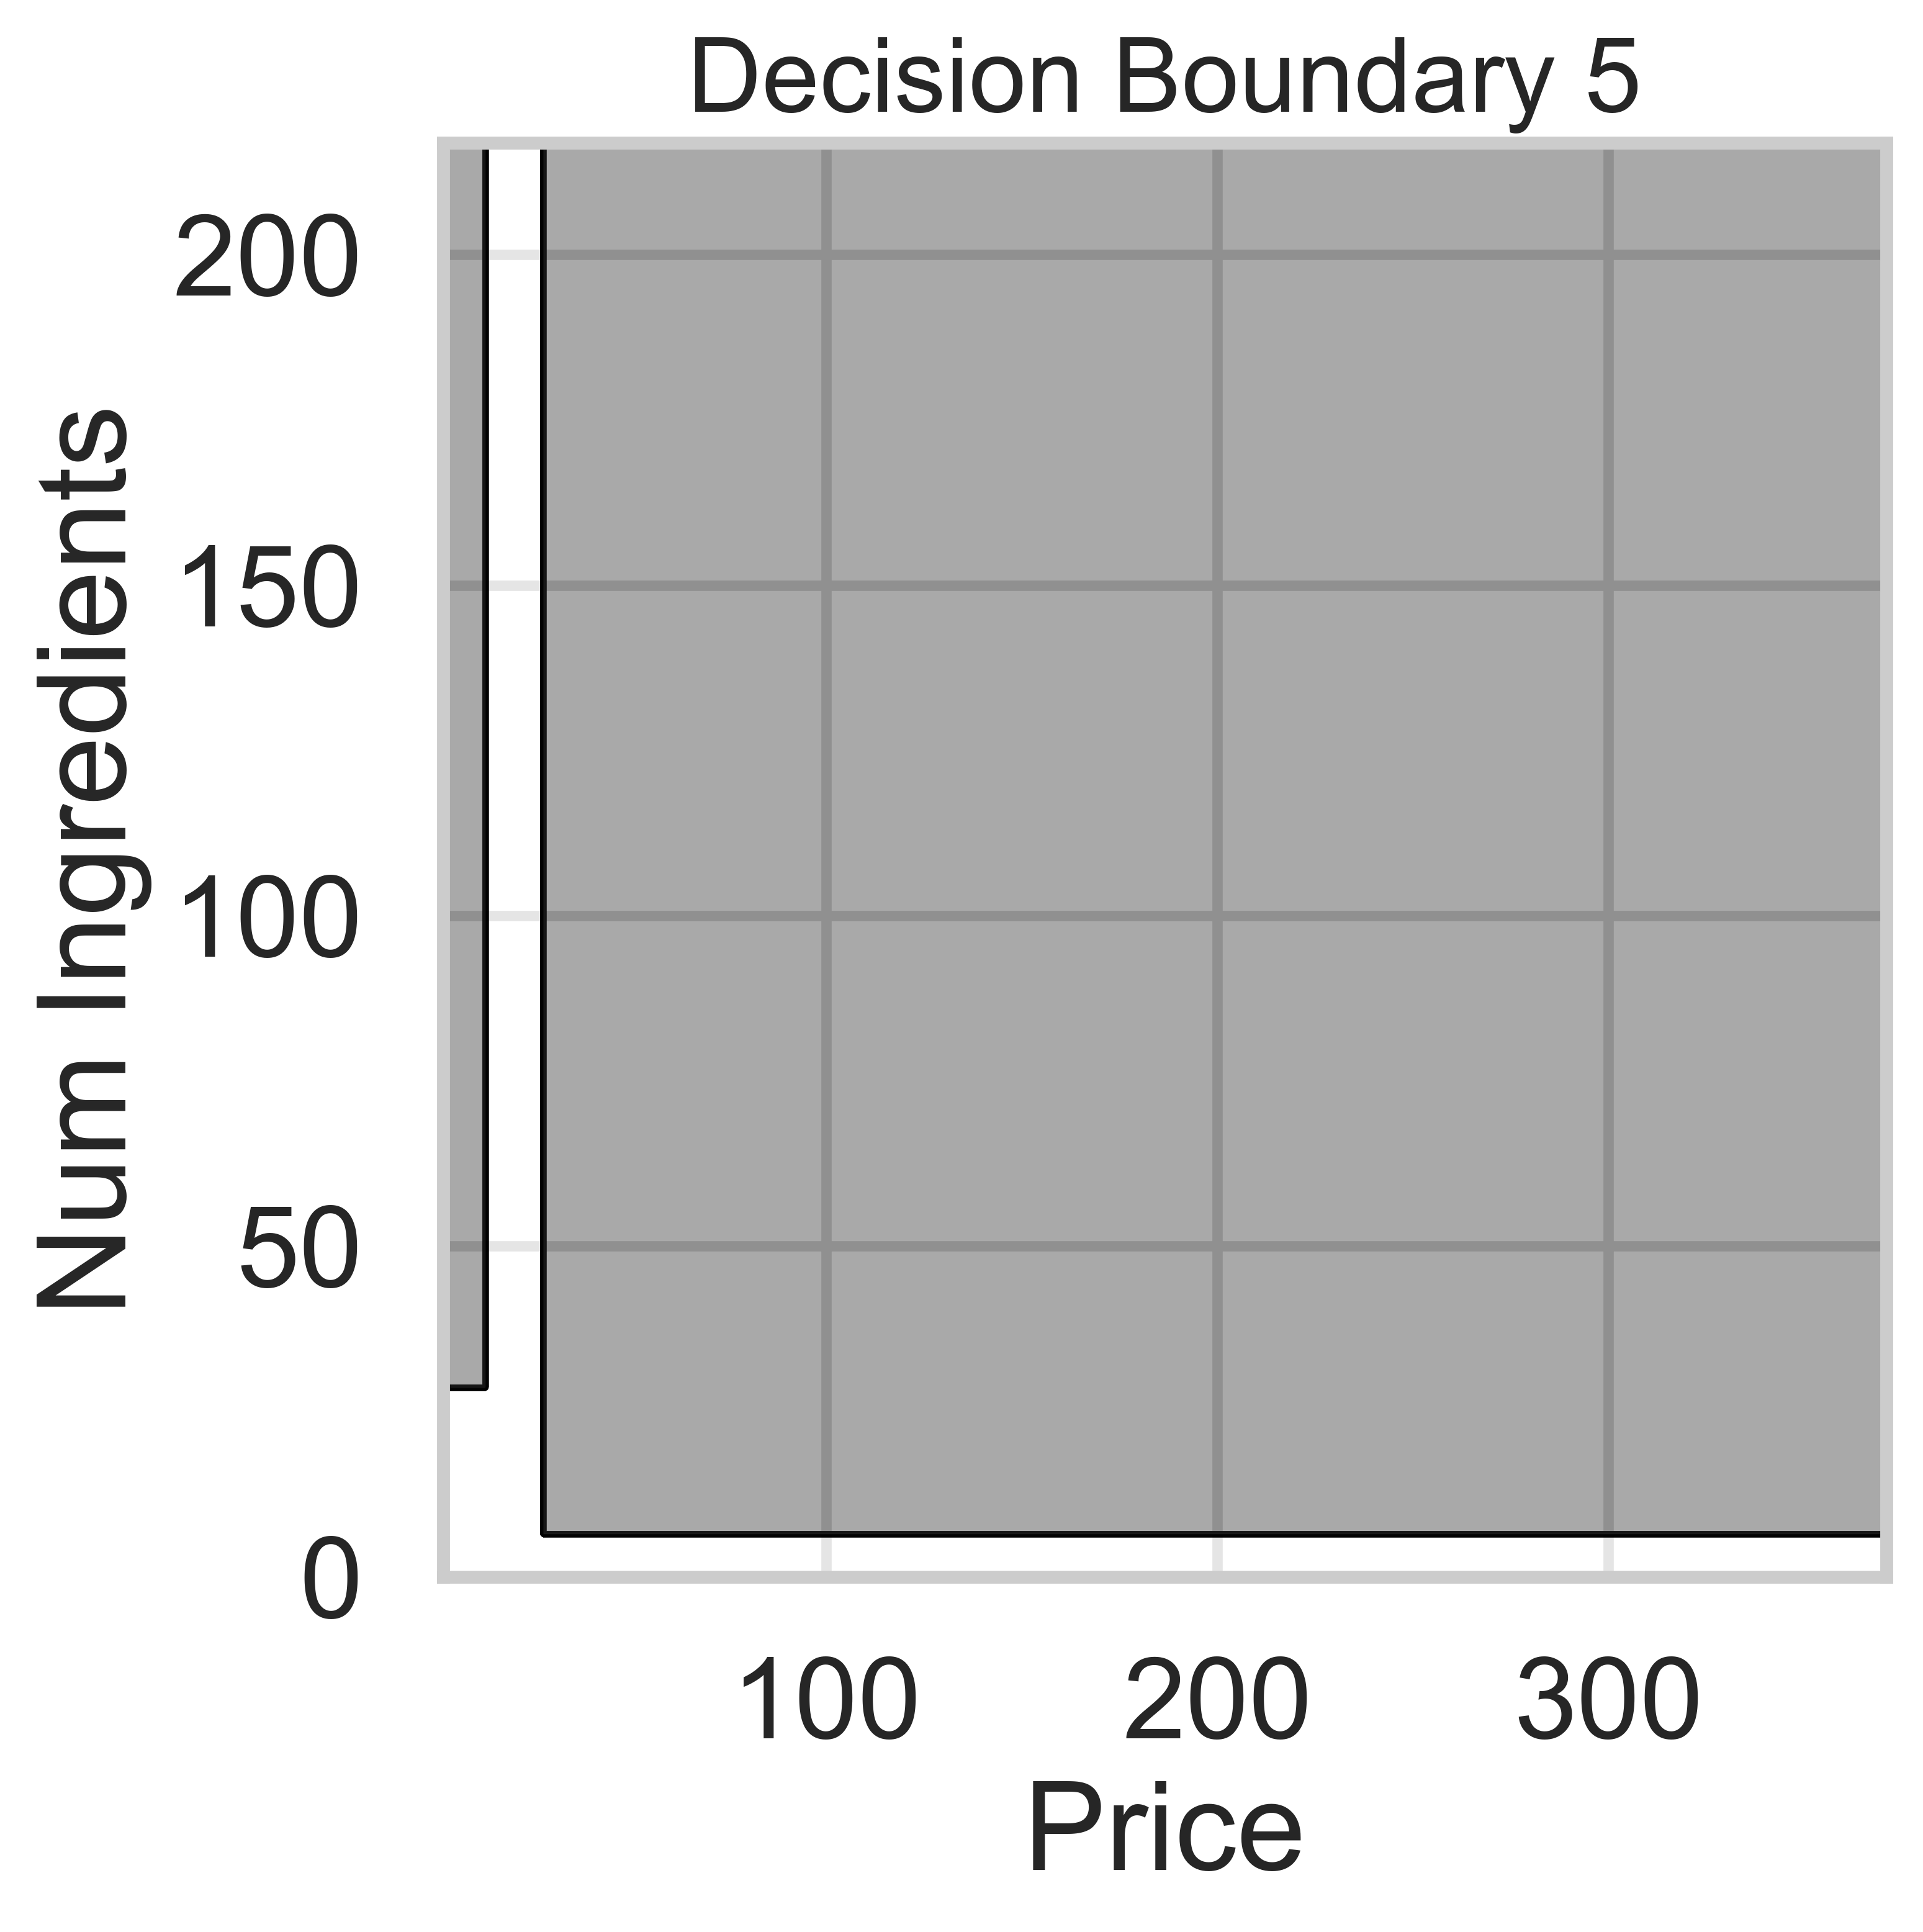
\includegraphics[width=\linewidth]{final-images/db5.png}
    \end{minipage}
\end{figure}

\begin{subprobset}

\begin{subprob}(1.5 pts) Which model does Decision Boundary 1 correspond to?

\begin{tabular}{ll}

\bubble{$k$-nearest neighbors with $k = 3$}

\bubble{$k$-nearest neighbors with $k = 100$}

\bubble{Decision tree with $\text{max depth} = 3$}

\bubble{Decision tree with $\text{max depth} = 15$}

\bubble{Logistic regression}

\end{tabular}

\end{subprob}

\begin{subprob}(1.5 pts) Which model does Decision Boundary 2 correspond to?

\begin{tabular}{ll}

\bubble{$k$-nearest neighbors with $k = 3$}

\bubble{$k$-nearest neighbors with $k = 100$}

\bubble{Decision tree with $\text{max depth} = 3$}

\bubble{Decision tree with $\text{max depth} = 15$}

\bubble{Logistic regression}

\end{tabular}

\end{subprob}

\begin{subprob}(1.5 pts) Which model does Decision Boundary 3 correspond to?

\begin{tabular}{ll}

\bubble{$k$-nearest neighbors with $k = 3$}

\bubble{$k$-nearest neighbors with $k = 100$}

\bubble{Decision tree with $\text{max depth} = 3$}

\bubble{Decision tree with $\text{max depth} = 15$}

\bubble{Logistic regression}

\end{tabular}

\end{subprob}

\begin{subprob}(1.5 pts) Which model does Decision Boundary 4 correspond to?

\begin{tabular}{ll}

\bubble{$k$-nearest neighbors with $k = 3$}

\bubble{$k$-nearest neighbors with $k = 100$}

\bubble{Decision tree with $\text{max depth} = 3$}

\bubble{Decision tree with $\text{max depth} = 15$}

\bubble{Logistic regression}

\end{tabular}

\end{subprob}

\end{subprobset}

\end{prob}

\newpage

\begin{prob}[(10 pts)]

Suppose we fit a logistic regression model that predicts whether a product is designed for sensitive skin, given its price, $x^{(1)}$, number of ingredients, $x^{(2)}$, and rating, $x^{(3)}$. After minimizing average cross-entropy loss, the optimal parameter vector is as follows:

$$\vec{w}^* = \begin{bmatrix} -1 \\ 1 / 5 \\ - 3 / 5 \\ 0 \end{bmatrix}$$

In other words, the intercept term is $-1$, the coefficient on price is $\frac{1}{5}$, the coefficient on the number of ingredients is $-\frac{3}{5}$, and the coefficient on rating is $0$.

Consider the following four products:

\vspace{-0.2in}

\begin{itemize}
    \item \textbf{Wolfcare}: Costs \$15, made of 20 ingredients, 4.5 rating
    \item \textbf{Go Blue Glow}: Costs \$25, made of 5 ingredients, 4.9 rating
    \item \textbf{DataSPF}: Costs \$50, made of 15 ingredients, 3.6 rating
    \item \textbf{Maize Mist}: Free, made of 1 ingredient, 5.0 rating
\end{itemize}

\vspace{-0.1in}

% \begin{subprobset}

% \begin{subprob}

Which of the following products have a predicted probability of being designed for sensitive skin of \textbf{at least 0.5 (50\%)}? For each product, select Yes or No and justify your answer.

\begin{adjustwidth}{-0.3in}{-0.3in} % Reduce margins by 1 inch on both sides
\begin{center}
\begin{minipage}[t]{0.53\textwidth}
    \vspace{-0.1in}
    \begin{center}
    \textbf{Wolfcare:}
    \bubble{Yes}
    \bubble{No}
    \end{center}
    \vspace{-0.1in}
    \begin{responsebox}{1.6in}
        
    \end{responsebox}
\end{minipage}
\hfill
\begin{minipage}[t]{0.53\textwidth}
    \vspace{-0.1in}
    \begin{center}
    \textbf{Go Blue Glow:}
    \bubble{Yes}
    \bubble{No}
    \end{center}
    \vspace{-0.1in}
    \begin{responsebox}{1.6in}
        
    \end{responsebox}
\end{minipage}

\vspace{0.2in}

\begin{minipage}[t]{0.53\textwidth}
    \vspace{-0.1in}
    \begin{center}
    \textbf{DataSPF:}
    \bubble{Yes}
    \bubble{No}
    \end{center}
    \vspace{-0.1in}
    \begin{responsebox}{1.6in}
        
    \end{responsebox}
\end{minipage}
\hfill
\begin{minipage}[t]{0.53\textwidth}
    \vspace{-0.1in}
    \begin{center}
    \textbf{Maize Mist:}
    \bubble{Yes}
    \bubble{No}
    \end{center}
    \vspace{-0.1in}
    \begin{responsebox}{1.6in}
        
    \end{responsebox}
\end{minipage}
\end{center}
\end{adjustwidth}
% \textbf{Wolfcare:}
% \vspace{-0.1in}
% \begin{center}
%     \bubble{Yes} \ \ \  \bubble{No}    
% \end{center}
% \vspace{-0.1in}
% \begin{responsebox}{0.75in}
    
% \end{responsebox}

% \textbf{Go Blue Glow:}
% \vspace{-0.1in}
% \begin{center}
%     \bubble{Yes} \ \ \  \bubble{No}    
% \end{center}
% \vspace{-0.1in}
% \begin{responsebox}{0.75in}
    
% \end{responsebox}

% \textbf{DataSPF:}
% \vspace{-0.1in}
% \begin{center}
%     \bubble{Yes} \ \ \  \bubble{No}    
% \end{center}
% \vspace{-0.1in}
% \begin{responsebox}{0.75in}
    
% \end{responsebox}

% \textbf{Maize Mist:}
% \vspace{-0.1in}
% \begin{center}
%     \bubble{Yes} \ \ \  \bubble{No}    
% \end{center}
% \vspace{-0.1in}
% \begin{responsebox}{0.75in}
    
% \end{responsebox}

% \end{subprob}

\vspace{0.15in}

% {\small You may use the space below for scratch work, but we will \textbf{not} grade anything below.}

% \vspace{0.2in}

\vspace{3.5in}

% \begin{subprob}

% In one English sentence, name one benefit of using cross-entropy loss instead of squared loss for logistic regression.

% \begin{responsebox}{1.25in}
    
% \end{responsebox}

% \end{subprob}

% \begin{enumerate}[label=(\roman*)]

% \item Suppose Wolfcare \textbf{is} designed for sensitive skin (i.e., the true $y$-value is 1). What is the cross-entropy loss of our model's prediction?

% \bubble{}

% \item Supoose Wolfcare \textbf{is not} designed for sensitive skin (i.e., the true $y$-value is 0). What is the cross-entropy loss of our model's prediction?

% \end{enumerate}

% \begin{subprob}

% One product above has a predicted probability of exactly 50\%. Which product is it?

% \bubble{Wolfcare} \bubble{Go Blue Glow} \bubble{DataSPF} \bubble{Maizyserum}

% \end{subprob}

% \end{subprobset}

\end{prob}

\newpage

\begin{prob}[(8 pts)]

Suppose, again, that we fit a logistic regression model that predicts whether a product is designed for sensitive skin. We're deciding between three thresholds, $A$, $B$, and $C$, all of which are real numbers between 0 and 1 (inclusive). If a product's predicted probability of being designed for sensitive skin is above our chosen threshold, we predict they belong to class 1 (yes); otherwise, we predict class 0 (no).

The confusion matrices of our model on the test set for all three thresholds are shown below.

\vspace{-0.3in}

\[
\begin{array}{ccc}
\textbf{$A$} & \textbf{$B$} & \textbf{$C$} \\
\begin{array}{|l|c|c|}
\hline
& \text{Pred.} \: 0 & \text{Pred.} \: 1 \\
\hline
\text{Actually} \: 0 & 40 & 5 \\
\hline
\text{Actually} \: 1 & 35 & 35 \\
\hline
\end{array}
&
\begin{array}{|l|c|c|}
\hline
& \text{Pred.} \: 0 & \text{Pred.} \: 1 \\
\hline
\text{Actually} \: 0 & 5 & 40 \\
\hline
\text{Actually} \: 1 & 10 & ??? \\
\hline
\end{array}
&
\begin{array}{|l|c|c|}
\hline
& \text{Pred.} \: 0 & \text{Pred.} \: 1 \\
\hline
\text{Actually} \: 0 & 10 & 35 \\
\hline
\text{Actually} \: 1 & 30 & 40 \\
\hline
\end{array}
\end{array}
\]

\begin{subprobset}

\begin{subprob}(2 pts) Suppose we choose threshold {$A$}, i.e. the \textbf{leftmost} confusion matrix. What is the precision of the resulting predictions? Give your answer as an \textbf{unsimplified fraction}.

\biginlineresponsebox[1.5in]{}

\end{subprob}

\begin{subprob}(1 pt) What is the missing value (???) in the confusion matrix for threshold $B$? Give your answer as an \textbf{integer}.

\inlineresponsebox[1.5in]{}

\end{subprob}

\begin{subprob}(3 pts) Using the information in the three confusion matrices, arrange the thresholds from \textbf{largest to smallest}. Remember that $0 \leq A, B, C \leq 1$.

\begin{tabular}{l@{\hspace{0pt}}l}

\bubble{$A$ $>$ $B$ $>$ $C$}

\bubble{$A$ $>$ $C$ $>$ $B$}

\bubble{$B$ $>$ $A$ $>$ $C$}

\bubble{$B$ $>$ $C$ $>$ $A$}

\bubble{$C$ $>$ $A$ $>$ $B$}

\bubble{$C$ $>$ $B$ $>$ $A$}
\end{tabular}

\end{subprob}

\begin{subprob}(2 pts) Remember that in our classification problem, class 1 means the product \textbf{is} designed for sensitive skin, and class 0 means the product \textbf{is not} designed for sensitive skin. In one or two English sentences, explain which is \textbf{worse} in this context and \textbf{why}: a false positive or a false negative.

\begin{responsebox}{1.5in}

A false positive is worse, as it would mean we predict a product is safe when it isn't; someone with sensitive skin may use it and it could harm them.

\end{responsebox}

\end{subprob}

\end{subprobset}

\end{prob}

\newpage

\begin{prob}[(5 pts)]

Let $\vec{x} = \begin{bmatrix} x_1 \\ x_2 \end{bmatrix}$. Consider the function $\displaystyle Q(\vec x) = x_1^2 - 2x_1x_2 + 3x_2^2 - 1$.

\begin{subprobset}

\begin{subprob}(3 pts) Fill in the blank to complete the definition of $\nabla Q(\vec x)$, the gradient of $Q$.

$$\nabla Q(\vec x) = \begin{bmatrix} 2(x_1 - x_2) \\ \\ \_\_\_\_ \end{bmatrix}$$

What goes in the blank? Show your work, and put a \boxed{\text{box}} your final answer, which should be an \textbf{expression involving $x_1$ and/or $x_2$}.

\begin{responsebox}{2in}
    
\end{responsebox}

\end{subprob}

\begin{subprob}(2 pts) We decide to use gradient descent to minimize $Q$, using an initial guess of $\vec x^{(0)} = \begin{bmatrix} 1 \\ 1 \end{bmatrix}$ and a learning rate/step size of $\alpha$.

If after one iteration of gradient descent, we have $\vec{x}^{(1)} = \begin{bmatrix} 1 \\ -4 \end{bmatrix}$, what is $\alpha$?

\vspace{0.1in}

\bubble{$\displaystyle \frac{1}{4}$}

\bubble{$\displaystyle \frac{1}{2}$}

\bubble{$\displaystyle \frac{3}{4}$}

\bubble{$\displaystyle \frac{5}{4}$}

\bubble{$\displaystyle \frac{3}{2}$}

\bubble{$\displaystyle \frac{5}{2}$}

\end{subprob}

\end{subprobset}

\end{prob}

\newpage

% \begin{prob}

% Suppose \texttt{k} is some positive integer such that:

% \begin{verbatim}
% >>> reviews.iloc[np.arange(-k, k, 3)].shape[0]
% 19
% \end{verbatim}

% What is the value of \texttt{k}?

% \bubble{\texttt{27}} \bubble{\texttt{28}} \bubble{\texttt{29}} \bubble{\texttt{30}} \bubble{\texttt{31}} \bubble{\texttt{32}} \bubble{\texttt{33}}
    
% \end{prob}

\begin{prob}[(4 pts)]

What is one topic from the second half of the semester that you studied a lot for but wasn't on the exam? \textbf{Blank answers will receive no credit!}

\begin{responsebox}{1.5in}

\end{responsebox}

\end{prob}

\vspace{0.5in}

% \newpage

\textbf{Make sure you've written your uniqname in the space provided in the top right corner of every page of this exam!}

Congrats on finishing the course --- we'll miss you! Feel free to draw us a picture about EECS 398 below :)

% (1 pt) And here's a free point!

\begin{responsebox}{4.5in}
    
\end{responsebox}

\end{probset}

\end{document}
